\chapter{Bending Members}
Beams are generally horizontal members supporting vertical loads and sometimes also frame lateral effects (e.g., from wind and earthquakes).
\begin{figure}[H]
\centering\includegraphics{PIC/CH05/BM}
\end{figure}
\section{Limit States}
The limit states of a bending member may consist of the following aspects.
\begin{itemize}
\item strength
\begin{itemize}
\item flexural
\begin{itemize}
\item section
\begin{itemize}
\item yielding
\item local buckling
\end{itemize}
\item member lateral buckling
\begin{itemize}
\item FLT buckling with residual stress
\item FLT buckling with warping
\end{itemize}
\end{itemize}
\item shear
\begin{itemize}
\item yielding
\item buckling
\end{itemize}
\item concentrated load
\begin{itemize}
\item yielding
\item buckling
\end{itemize}
\end{itemize}
\item serviceability
\begin{itemize}
\item excessive deflection
\item excessive vibration
\end{itemize}
\end{itemize}
Interaction may occur between limit states (e.g., beam yielding and local buckling). Such interactions should be considered in design. The only requirement for a well designed beam is that: \emph{The capacity must be greater than the demands for each limit state.}

The most efficient beams to carry flexure are those with the areas of steel in tension and compression as far apart as possible. The limit states above, and constructability/installation/cost issues give limit the practical sizes that can be used.

We will look at the limit states in turn.
\begin{figure}[H]
\centering
\includegraphics[width=.99\textwidth]{PIC/CH05/CA}
\caption{Critical areas for consideration of web stiffeners \citep{Gorenc2015}}
\end{figure}
\section{Section Flexural Yielding Strength}
We often adopt the \textbf{elastic perfectly plastic} idealisation for steel material response.
\begin{figure}[H]
\centering
\footnotesize
\begin{tikzpicture}[scale=.6]
\begin{scope}
\draw[->](0,0)--(8,0)node[below=2mm]{strain};
\draw[->](0,0)--(0,5)node[left=2mm]{stress};
\draw[very thick,line join=round](0,0)--(1,4)--(1.02,3.5)(4,3.5)to[out=30,in=180](6,4.2)to[out=0,in=160](8,3.8);
\draw[very thick,line join=round,decoration={random steps,segment length=2pt,amplitude=1.5pt}]decorate{(1.02,3.5)--(4,3.5)};
\node at(4,2){typical response};
\end{scope}
\begin{scope}[xshift=12cm]
\draw[->](0,0)--(8,0)node[below=2mm]{strain};
\draw[->](0,0)--(0,5)node[left=2mm]{stress};
\draw[very thick,line join=round](0,0)--(.875,3.5)--(8,3.5);
\node[align=center]at(4,2){idealised response\\elastic perfectly plastic};
\draw[dashed](.875,3.5)--(0,3.5)node[left=2mm]{$f_y$};
\draw[dashed](.875,3.5)--(.875,0)node[below=2mm]{$\varepsilon_y$};
\draw(.875*.3,3.5*.3)node[circle,fill=cc0066]{}node[left=2mm]{(a)};
\draw(.875,3.5)node[circle,fill=cc0066]{}node[above=2mm]{(b)};
\draw(2.5,3.5)node[circle,fill=cc0066]{}node[above=2mm]{(c)};
\draw(6,3.5)node[circle,fill=cc0066]{}node[above=2mm]{(d)};
\end{scope}
\end{tikzpicture}
\caption{Idealisation of steel response}
\end{figure}

The development of plasticity of a rectangular section subject to increasing bending can thus be illustrated as follows. The material responses of extreme fibres, that correspond to four states, are labelled in the above figure as well.
\begin{figure}[H]
\centering
\footnotesize
\begin{tikzpicture}
\newcommand{\Base}[1]{\clip(-1.5,-.5)rectangle(1.5,2.5);
\draw[dashed](-.8,0)--++(0,2)node[above]{$-\varepsilon_y$}(.8,0)--++(0,2)node[above]{$\varepsilon_y$};
\draw[fill=cc0066,opacity=.4](0,0)--(0,2)--(#1,2)--(-#1,0)--cycle;}
\begin{scope}
\Base{0.2}
\end{scope}
\begin{scope}[xshift=4cm]
\Base{0.8}
\end{scope}
\begin{scope}[xshift=8cm]
\Base{1.2}
\end{scope}
\begin{scope}[xshift=12cm]
\Base{40}
\end{scope}
\renewcommand{\Base}{\draw[dashed](-.8,0)--++(0,2)node[above]{$-f_y$}(.8,0)--++(0,2)node[above]{$f_y$};}
\begin{scope}[yshift=-3cm]
\begin{scope}
\Base
\draw[fill=0066cc,opacity=.4](0,0)--(0,2)--(.2,2)--(-.2,0)--cycle;
\end{scope}
\begin{scope}[xshift=4cm]
\Base
\draw[fill=0066cc,opacity=.4](0,0)--(0,2)--(.8,2)--(-.8,0)--cycle;
\end{scope}
\begin{scope}[xshift=8cm]
\Base
\draw[fill=0066cc,opacity=.4](0,0)|-(.8,2)--(.8,1.75)--(-.8,.25)|-cycle;
\end{scope}
\begin{scope}[xshift=12cm]
\Base
\draw[fill=0066cc,opacity=.4](0,0)|-(.8,2)|-(-.8,1)|-cycle;
\end{scope}
\end{scope}
\renewcommand{\Base}[2]{\draw[ultra thick](-.8,0)rectangle(.8,2);
\draw[pattern=north west lines](-.8,0)rectangle(.8,1-#1);
\draw[pattern=north west lines](-.8,2)rectangle(.8,1+#1);
\node[align=center]at(0,-.7){#2};
}
\begin{scope}[yshift=-6cm]
\begin{scope}
\Base{1}{$M<M_y$\\(a)};
\end{scope}
\begin{scope}[xshift=4cm]
\Base{1}{$M=M_y$\\(b)};
\end{scope}
\begin{scope}[xshift=8cm]
\Base{.5}{$M_y<M<M_p$\\(c)};
\end{scope}
\begin{scope}[xshift=12cm]
\Base{0}{$M=M_p$\\(d)};
\end{scope}
\end{scope}
\end{tikzpicture}
\caption{Development of plasticity of a rectangular section}
\end{figure}
\begin{figure}[H]
\centering
\begin{tikzpicture}
\begin{scope}
\node at(-1,0){(a)};
\draw(0,-.6)rectangle(6,.6);
\begin{scope}[xshift=8cm]
\draw[very thick,fill=black!10](0,.6)--++(6,0)--++(-3,-.4)--cycle;
\draw[dashed](2,-.1)--++(2,0)node[right=4mm]{$M_y$};
\draw[dashed](2,-.6)--++(2,0)node[right=4mm]{$M_p$};
\end{scope}
\end{scope}
\begin{scope}[yshift=-2cm]
\node at(-1,0){(b)};
\draw(0,-.6)rectangle(6,.6);
\draw(3,-.6)node[fill,circle,inner sep=0,minimum size=1mm]{};
\draw(3,.6)node[fill,circle,inner sep=0,minimum size=1mm]{};
\begin{scope}[xshift=8cm]
\draw[very thick,fill=black!10](0,.6)--++(6,0)--++(-3,-.7)--cycle;
\draw[dashed](2,-.1)--++(2,0)node[right=4mm]{$M_y$};
\draw[dashed](2,-.6)--++(2,0)node[right=4mm]{$M_p$};
\end{scope}
\end{scope}
\begin{scope}[yshift=-4cm]
\node at(-1,0){(c)};
\draw(0,-.6)rectangle(6,.6);
\draw[pattern=north west lines](2,.6)--++(2,0)--++(-1,-.2)--cycle;
\draw[pattern=north west lines](2,-.6)--++(2,0)--++(-1,.2)--cycle;
\begin{scope}[xshift=8cm]
\draw[very thick,fill=black!10](0,.6)--++(6,0)--++(-3,-.9)--cycle;
\draw[dashed](2,-.1)--++(2,0)node[right=4mm]{$M_y$};
\draw[dashed](2,-.6)--++(2,0)node[right=4mm]{$M_p$};
\end{scope}
\end{scope}
\begin{scope}[yshift=-6cm]
\node at(-1,0){(d)};
\draw(0,-.6)rectangle(6,.6);
\draw[pattern=north west lines](1.5,.6)--++(3,0)--++(-1.5,-.6)--cycle;
\draw[pattern=north west lines](1.5,-.6)--++(3,0)--++(-1.5,.6)--cycle;
\begin{scope}[xshift=8cm]
\draw[very thick,fill=black!10](0,.6)--++(6,0)--++(-3,-1.2)--cycle;
\draw[dashed](2,-.1)--++(2,0)node[right=4mm]{$M_y$};
\draw[dashed](2,-.6)--++(2,0)node[right=4mm]{$M_p$};
\end{scope}
\end{scope}
\end{tikzpicture}
\caption{Development of plasticity of a rectangular section in a beam}
\end{figure}
Denote the height and width of the section to be $h$ and $b$, the yield moment $M_y$ and plastic moment $M_p$ can be computed as
\begin{gather*}
M_y=\dfrac{bh^2}{6}f_y=Zf_y,\qquad
M_p=\dfrac{bh^2}{4}f_y=Sf_y,
\end{gather*}
where $Z$ and $S$ are elastic and plastic section moduli. Note in \ANSI{}, $S$ is used for elastic section modulus and $Z$ is used for plastic section modulus, in Eurocode 3, $W_{el}$ and $W_{pl}$ are used. No matter which convention is used, the plastic section modulus is always greater than the elastic section modulus.
\begin{figure}[H]
\centering
\begin{tikzpicture}
\draw[dashed](-6,0)--(6,0);
\draw[dashed](0,1.5)--(0,-6);
\draw[|<->|](0,-1)--(0,0)node[midway,fill=white]{$h/2$};
\draw[|<->|](0,1)--(0,0)node[midway,fill=white]{$h/2$};
\draw[|<->|](1,.5)--(1,0)node[midway,fill=white,right=4mm]{$h/4$};
\draw[|<->|](-1,-.67)--(-1,0)node[midway,fill=white,left=4mm]{$h/3$};
\begin{scope}[xshift=-3cm]
\draw[dashed](0,-1.5)--++(0,3);
\draw[fill=black!20](0,-1)|-++(1,2)--++(-2,-2)--cycle;
\draw[ultra thick,,<-](0,.67)--++(1.5,0)node[fill=white,anchor=west]{$F_y$};
\draw[ultra thick,<-](0,-.67)--++(-1.5,0)node[fill=white,anchor=east]{$F_y=f_y\times\dfrac{bh}{2}$};
\node at(0,-2){elastic};
\node[anchor=north,align=left]at(0,-3){$M_y=2\times{}F_y\times\dfrac{h}{3}$\\[3mm]$M_y=2\times{}f_y\times\dfrac{bh}{4}\times\dfrac{h}{3}$\\[3mm]$M_y=\dfrac{bh^2}{6}f_y$};
\end{scope}
\begin{scope}[xshift=3cm]
\draw[dashed](0,-1.5)--++(0,3);
\draw[fill=black!20](-1,-1)|-++(0,1)--++(2,0)--++(0,1)--++(-1,0)|-cycle;
\draw[ultra thick,<-](0,.5)--++(1.5,0)node[fill=white,anchor=west]{$F_p=f_y\times\dfrac{bh}{2}\times\dfrac{1}{2}$};
\draw[ultra thick,,<-](0,-.5)--++(-1.5,0)node[fill=white,anchor=east]{$F_p$};
\node at(0,-2){plastic};
\node[anchor=north,align=left]at(0,-3){$M_p=2\times{}F_p\times\dfrac{h}{4}$\\[3mm]$M_p=2\times{}f_y\times\dfrac{bh}{2}\times\dfrac{h}{4}$\\[3mm]$M_p=\dfrac{bh^2}{4}f_y$};
\end{scope}
\end{tikzpicture}
\end{figure}

The moduli $Z$ and $S$ for each section are given in the specification manual. Like form factor $k_f$, there is no need to calculate them in practice. The ratio between $S$ and $Z$ is defined as the shape factor.
\begin{gather*}
\mathrm{SF}=\dfrac{S}{Z}.
\end{gather*}
For rectangular sections, $\mathrm{SF}=1.5$. The value of shape factor would vary between \num{1} and \num{1.5} depending on different section shapes. As the shape factor increases, more of the length of the beam yields resulting in less concentration of the inelastic rotation, but a higher likelihood of element buckling instability.

If one plots section curvature versus moment, the following response can be obtained.
\begin{figure}[H]
\centering
\footnotesize
\begin{tikzpicture}[>=latex]
\begin{axis}[
declare function={normal(\x)=1.5*(\x/.3/(1+(\x/.3)^4)^0.25);},
width=10cm,
height=6cm,
xtick=\empty,
ytick=\empty,
axis x line=center,
axis y line=center,
xlabel={curvature},
ylabel={moment},
xlabel style={below right},
ylabel style={above left},
xmin=-.5,xmax=4,ymin=0,ymax=2]
\addplot[line width=.6mm,domain=0:3,samples=100]{normal(x)};
\draw[dashed](axis cs:2,1.5)--(axis cs:0,1.5)node[left]{$M_p$};
\draw[dashed](axis cs:.2,{normal(.2)})--(axis cs:0,{normal(.2)})node[left]{$M_y$};
\draw(.1,{normal(.1)})node[fill=cc0066,circle,inner sep=0,minimum size=2mm]{}node[right=2mm,fill=white]{(a)};
\draw(.2,{normal(.2)})node[fill=cc0066,circle,inner sep=0,minimum size=2mm]{}node[right=2mm,fill=white]{(b)};
\draw(.3,{normal(.3)})node[fill=cc0066,circle,inner sep=0,minimum size=2mm]{}node[right=2mm,fill=white]{(c)};
\draw(1,{normal(1)})node[fill=cc0066,circle,inner sep=0,minimum size=2mm]{}node[right=2mm,fill=white]{(d)};
\draw[dashed](.4,{normal(.4)})to[out=30,in=185](3.5,1.7)node[fill=white]{if hardening};
\end{axis}
\end{tikzpicture}\caption{Section response}
\end{figure}
If the section \textbf{does not buckle} and is \textbf{ductile}, then the section strength is closer to $M_p$ than to $M_y$. The fact that we have strain hardening in the steel means that $M_p$ can easily be obtained in actual members, although $M_p$ implies an infinite curvature with the steel model chosen.
\subsection{Calculation of Plastic Modulus}
The plastic modulus $S$ for random sections with uniform yield stress is essentially its \textbf{first moment of area}.
\begin{gather*}
S_x=\int_A|y|~\md{A},\qquad
S_y=\int_A|x|~\md{A},
\end{gather*}
where $x$ and $y$ are the perpendicular distances (lever arms) to the centroid of element $\md{A}$ from the corresponding plastic neutral axes.

The plastic neutral axis coincides with the centroid of section which splits the area into two equal halves.

It should be emphasised that the above statements are \textbf{only} valid for sections with uniform yield stress.
\section{Strength Considering Local Buckling}
Sections with high element slendernesses are likely to buckle before the plastic moment capacity is reached.

The slenderness of any \textbf{flat element} $i$ of the section for flexure, $\lambda_{e,i}$, is obtained in a similar way as it is for compression members (\NZSSTEEL{\S~5.2.2.1}):
\begin{gather*}
\lambda_{e,i}=\dfrac{b_i}{t_i}\sqrt{\dfrac{f_{y,i}}{\SI{250}{\mpa}}},
\end{gather*}
where $b_i$ is again the clear width of the element outstand from the face of the supporting plate element or the clear width of the element between the faces of supporting plate elements and $t_i$ is the element thickness.
\begin{figure}[H]
\centering
\begin{tikzpicture}[x=1cm,y=1cm,scale=.5]
\draw[fill=0066cc](-.25,-4.5)rectangle(.25,4.5);
\draw[fill=cc0066](-2.5,-4.5)rectangle(2.5,-4);
\draw[fill=cc0066](-2.5,4)rectangle(2.5,4.5);
\draw[fill=00cc66](-.25,4)rectangle(.25,4.5);
\draw[fill=00cc66](-.25,-4)rectangle(.25,-4.5);
\draw[|<->|](3,-4)--++(0,8)node[midway,fill=white]{$b_5$};
\draw[|<->|](-.25,-5)--++(.5,0)node[midway,fill=white,below=3mm]{$t_5$};
\draw[|<->|](-2.5,5.5)--++(2.25,0)node[midway,fill=white]{$b_1$};
\draw[|<->|](2.5,5.5)--++(-2.25,0)node[midway,fill=white]{$b_2$};
\draw[|<->|](-2.5,-5.5)--++(2.25,0)node[midway,fill=white]{$b_3$};
\draw[|<->|](2.5,-5.5)--++(-2.25,0)node[midway,fill=white]{$b_4$};
\draw[|<->|](3,4)--++(0,.5)node[midway,fill=white,right=3mm]{$t_1,t_2$};
\draw[|<->|](3,-4)--++(0,-.5)node[midway,fill=white,right=3mm]{$t_3,t_4$};
\begin{scope}[xshift=14cm]
\draw[fill=0066cc](-4,-4)rectangle(4,4);
\draw[fill=cc0066](-4,-4)rectangle++(.4,.4);
\draw[fill=cc0066](4,-4)rectangle++(-.4,.4);
\draw[fill=cc0066](4,4)rectangle++(-.4,-.4);
\draw[fill=cc0066](-4,4)rectangle++(.4,-.4);
\draw[fill=white](-3.6,-3.6)rectangle(3.6,3.6);
\draw[|<->|](4.4,-3.6)--(4.4,3.6)node[midway]{$b_6$};
\draw[|<->|](3.6,-4.5)--(4,-4.5)node[midway,right]{$t_6$};
\draw[|<->|](-3.6,4.5)--(3.6,4.5)node[midway,above]{$b_7$};
\draw[|<->|](-4.4,3.6)--(-4.4,4)node[midway,left]{$t_7$};
\end{scope}
\end{tikzpicture}
\caption{Flat elements in different sections}
\end{figure}

The slenderness for the \textbf{whole section} $\lambda_s$ is set to $\lambda_e$ for the element with the \textbf{greatest} ratio of $\lambda_e/\lambda_{ey}$. Similarly, the slenderness limits for the whole section $\lambda_{sp}$ and $\lambda_{sy}$ are taken as $\lambda_{ep}$ and $\lambda_{ey}$ for the element with the greatest ratio of $\lambda_e/\lambda_{ey}$. The element slenderness limits $\lambda_{ep}$ and $\lambda_{ey}$ are given in \tabref{tab:yield_limit} (\NZSSTEEL{Table~5.2}).
\begin{table}[htbp]
\centering\footnotesize
\caption{Values of slenderness limits for flat elements}\label{tab:yield_limit}
\begin{tabular}{ccc|ccc}
	\toprule
	\parbox{2.5cm}{\centering{}longitudinal edges supported} & \parbox{2cm}{\centering{}compression distribution} &  residual stress   & $\lambda_{ep}$ & $\lambda_{ey}$ & $\lambda_{ed}$ \\ \midrule
	                \multirow{8}[0]{*}{one}                  &            \multirow{4}[0]{*}{uniform}             &         SR         &       10       &       16       &       35       \\
	                                                         &                                                    &         HR         &       9        &       16       &       35       \\
	                                                         &                                                    &       LW, CF       &       8        &       15       &       35       \\
	                                                         &                                                    &         HW         &       8        &       14       &       35       \\
	                     \cmidrule{2-6}                      &            \multirow{4}[0]{*}{gradient}            &         SR         &       10       &       25       &                \\
	                                                         &                                                    &         HR         &       9        &       25       &                \\
	                                                         &                                                    &       LW, CF       &       8        &       22       &                \\
	                                                         &                                                    &         HW         &       8        &       22       &                \\ \midrule
	                \multirow{6}[0]{*}{both}                 &            \multirow{4}[0]{*}{uniform}             &         SR         &       30       &       45       &       90       \\
	                                                         &                                                    &         HR         &       30       &       45       &       90       \\
	                                                         &                                                    &       LW, CF       &       30       &       40       &       90       \\
	                                                         &                                                    &         HW         &       30       &       35       &       90       \\
	                     \cmidrule{2-6}                      &            \multirow{2}[0]{*}{gradient}             & Web of RHS and SHS &       45       &       60       &                \\
	                                                         &                                                    &       Other        &       85       &      130       &                \\ \bottomrule
\end{tabular}
\end{table}

The following are some examples on different cases of supported edges and compression distributions.
\begin{itemize}
\item For flanges of I sections subject to strong axis bending, only \textbf{one} edge is supported, both ends experience the same magnitude of normal stress, thus the compression distribution pattern is \textbf{uniform}. For HR sections, $\lambda_{ep}=9$ and $\lambda_{ey}=16$.
\begin{figure}[H]
\centering
\input{PIC/CH05/SR1}
\end{figure}
\item For web of I sections subject to strong axis bending, \textbf{both} edges are supported, one end experiences compression while the other experiences tension, thus the compression distribution pattern is \textbf{gradient}. For HR sections, $\lambda_{ep}=85$ and $\lambda_{ey}=130$.
\begin{figure}[H]
\centering
\input{PIC/CH05/SR2}
\end{figure}
\item For flanges of I sections subject to weak axis bending, only \textbf{one} edge is supported, but one end experiences compression/tension while the other has zero normal stress, thus the compression distribution pattern is \textbf{gradient}. For HR sections, $\lambda_{ep}=9$ and $\lambda_{ey}=25$.
\begin{figure}[H]
\centering
\input{PIC/CH05/SR3}
\end{figure}
\item For flanges of RHS/SHS sections subject to strong axis bending, \textbf{both} edges are supported, both ends experience the same magnitude of normal stress, thus the compression distribution pattern is \textbf{uniform}. For HW sections, $\lambda_{ep}=30$ and $\lambda_{ey}=35$.
\begin{figure}[H]
\centering
\begin{tikzpicture}
\draw[dashed](-2,0)--(3,0);
\draw[dashed](2,-1.5)--++(0,3);
\draw[fill=black!20](2,-1)|-++(1,2)--++(-2,-2)--cycle;
\draw[line width=2mm,black!20](-2,-1)rectangle++(2,2);
\draw[line width=2mm,cc0066](-1.9,1)--(-.1,1)(-1.9,-1)--(-.1,-1);
\end{tikzpicture}
\end{figure}
\item For webs of RHS/SHS sections subject to strong axis bending, \textbf{both} edges are supported, one end experiences compression while the other experiences tension, thus the compression distribution pattern is \textbf{gradient}. Thus, $\lambda_{ep}=45$ and $\lambda_{ey}=60$.
\begin{figure}[H]
\centering
\begin{tikzpicture}
\draw[dashed](-2,0)--(6,0);
\draw[dashed](2,-1.5)--++(0,3);
\draw[dashed](5,-1.5)--++(0,3);
\draw[fill=black!20](2,-1)|-++(1,2)--++(-2,-2)--cycle;
\draw[fill=black!20](4,-1)|-++(0,1)--++(2,0)--++(0,1)--++(-1,0)|-cycle;
\draw[line width=2mm,black!20](-2,-1)rectangle++(2,2);
\draw[line width=2mm,cc0066](-2,-.9)--(-2,.9)(0,-.9)--(0,.9);
\node at(2,-2){elastic};
\node at(5,-2){plastic};
\end{tikzpicture}
\end{figure}
\end{itemize}

Sections of different slendernesses are defined in the following way:
\begin{itemize}
\item $\lambda_s\leqslant\lambda_{sp}$ --- compact
\item $\lambda_{sp}<\lambda_s\leqslant\lambda_{sy}$ --- non-compact
\item $\lambda_{sy}<\lambda_s$ --- slender
\end{itemize}
The real behaviour of different types of sections, accounting for plastic material response, can be described in the following figure.
\begin{figure}[H]
\centering
\includegraphics{PIC/CH05/SECC}\caption{Flexural behaviour of different types of sections}
\end{figure}

The nominal section moment capacity $M_s$ shall be calculated as
\begin{gather}
M_s=f_yZ_e,
\end{gather}
where $Z_e$ is the effective section modulus which shall be determined by section type and section slenderness ratio.
\subsubsection{Compact Section ($M=M_c$)}
When section slenderness ratio is smaller than the section plasticity limit, $\lambda_s\leqslant\lambda_{sp}$, the section is \textbf{compact}, reaching a strength of $M_c=\min\left(M_p,~1.5M_y\right)$. \NZSSTEEL{\S~5.2.3} defines $Z_e$ to be the compact modulus $Z_c$ for compact sections, which shall be the smaller of $S$ and $1.5Z$. The compactness is given along with other section specifications.
\begin{gather}\label{eq:compact_modulus}
Z_e=Z_c=\min\left(S,~1.5Z\right).
\end{gather}

When holes exist, $S$ and $Z$ shall be recomputed considering holes (\NZSSTEEL{\S~5.2.7}).
\subsubsection{Non-compact Section ($M_y\leqslant{}M\leqslant{}M_c$)}
When section slenderness ratio is between the section plasticity and yield limits, $\lambda_{sp}<\lambda_s\leqslant\lambda_{sy}$, the section is \textbf{non-compact}. Then effective section modulus $Z_e$ shall be calculated via linear interpolation (\NZSSTEEL{\S~5.2.4}).
\begin{gather}
Z_e=Z+\dfrac{\lambda_{sy}-\lambda_s}{\lambda_{sy}-\lambda_{sp}}\left(Z_c-Z\right),
\end{gather}
where $Z_c$ is the compact modulus defined in \eqsref{eq:compact_modulus}.
\subsubsection{Slender Section ($M<M_y$)}
When section slenderness ratio is greater than the section yield limit, $\lambda_s>\lambda_{sy}$, the section is \textbf{slender}. For slender sections, many cases shall be considered. For simplicity, one can use the following expression (\NZSSTEEL{\S~5.2.5.2}) to calculate $Z_e$ as a conservative design.
\begin{gather}
Z_e=Z\left(\dfrac{\lambda_{sy}}{\lambda{s}}\right)^2.
\end{gather}
It shall be noted that slender sections are often not economical thus generally avoided.

If one plots $M_s$ against $\lambda_s$, the curve has a similar shape as seen in compression members in which elastic buckling is expected for slender sections, and residual stress effects control the behaviour. The effective section moduli $Z_e$ for both axes are also given in the specification.
\begin{figure}[H]
\centering\footnotesize
\begin{tikzpicture}[>=latex]
\begin{axis}[
width=10cm,
height=7cm,
xtick=\empty,
ytick=\empty,
axis x line=center,
axis y line=center,
xlabel={$\lambda_s$},
ylabel={$M_s$},
xlabel style={right},
ylabel style={left},
xmin=-1,xmax=4,ymin=-.2,ymax=1.2]
\addplot[line width=.6mm,domain=0:1,samples=100]{1};
\addplot[line width=.6mm,domain=1:2,samples=100]{-0.25*x+1.25};
\addplot[line width=.6mm,domain=2:4,samples=100]{3/x/x};
\draw[dashed](1,1)--(1,0)node[below]{$\lambda_{sp}$};
\draw[dashed](2,.75)--(2,0)node[below]{$\lambda_{sy}$};
\draw[dashed](1,1)--(0,1)node[left]{$M_cf_yZ_c$};
\draw[dashed](2,.75)--(0,.75)node[left]{$M_y=f_yZ$};
\node at(.5,.2){compact};
\node at(1.5,.2){non-compact};
\node at(2.5,.2){slender};
\end{axis}
\end{tikzpicture}\caption{Section capacity as a function of slenderness}
\end{figure}
\section{Strength Considering Member Buckling}
A bending member, like a compression member, may undergo lateral buckling. However, only the part of the section in compression has the tendency to buckle.
\begin{figure}[H]
\centering\begin{tikzpicture}
\node at(0,0){\includegraphics[width=10cm]{PIC/CH05/SS}};
\begin{scope}[xshift=8cm,scale=.3]
\draw[pattern=north west lines](-.25,0)rectangle(.25,4);
\draw[pattern=north west lines](-2.5,4)rectangle(2.5,4.5)node[above=4mm]{compression};
\draw[dashed](-.25,-4)rectangle(.25,4);
\draw[dashed](-2.5,-4.5)rectangle(2.5,-4);
\end{scope}
\end{tikzpicture}
\caption{Compression develops in the upper part of a beam}
\end{figure}
Beam buckling over its length is generally called Flexural Lateral Torsional (FLT) buckling. Because part of the section is in tension, and doesn't tend to buckle, it restrains the total connection.
\begin{figure}[H]
\centering\footnotesize
\begin{tikzpicture}[scale=.8]
\newcommand{\Base}[2]{\draw[#1](-1,-1.5)--++(2,0)(-1,1.5)--++(2,0)(0,-1.5)--++(0,3);
\node[inner sep=0,minimum size=0]at(0,-2.5){#2};}
\begin{scope}
\Base{dashed}{Flexural}
\begin{scope}[yshift=-.4cm]
\Base{line width=1.2mm}{}
\end{scope}
\end{scope}
\begin{scope}[xshift=5cm]
\Base{dashed}{Lateral}
\begin{scope}[xshift=.6cm]
\Base{line width=1.2mm}{}
\end{scope}
\end{scope}
\begin{scope}[xshift=10cm]
\Base{dashed}{Torsional}
\begin{scope}[rotate=-30]
\Base{line width=1.2mm}{}
\end{scope}
\end{scope}
\begin{scope}[xshift=15cm]
\Base{dashed}{FLT}
\begin{scope}[xshift=.6cm,yshift=-.4cm,rotate=-30]
\Base{line width=1.2mm}{}
\end{scope}
\end{scope}
\node at(2.5,0){\Huge$+$};
\node at(7.5,0){\Huge$+$};
\node at(12.5,0){\Huge$=$};
\end{tikzpicture}\caption{Components of FLT buckling}
\end{figure}

The amount of FLT buckling depends on
\begin{itemize}
\item slenderness of compression part of section
\item orientation of section
\item member length
\item member bracing type and positions
\item type and location of loading
\end{itemize}
Interested readers can check \href{https://www.youtube.com/watch?v=XSl7ZntK94E}{this}\footnote{\url{https://www.youtube.com/watch?v=XSl7ZntK94E}} video.
\subsection{Orientation Effect}
I sections bending about their strong axis with an unbraced compression flange are susceptible to buckling. However, strengths of other sections are not always affected by buckling. Lateral buckling is not generally significant in the following members.
\begin{figure}[H]
\centering\footnotesize
\begin{tikzpicture}[scale=.8]
\begin{scope}
\draw[line width=1.2mm](-1.5,-1)--++(0,2)(1.5,-1)--++(0,2)(-1.5,0)--++(3,0);
\draw[dashed](-2,0)--++(4,0);
\end{scope}
\begin{scope}[xshift=5cm]
\draw[line width=1.2mm](-1,-1)rectangle(1,1);
\draw[dashed](-2,0)--++(4,0);
\end{scope}
\begin{scope}[xshift=10cm]
\draw[line width=1.2mm](0,0)circle(1.2cm);
\draw[dashed](-2,0)--++(4,0);
\end{scope}
\end{tikzpicture}\caption{Sections less sensitive to lateral buckling}
\end{figure}
\subsection{Uniform Moment}
\subsubsection{Reference Moment}
From the mechanics of materials, it can be shown that the elastic buckling moment of a beam bending about its strong axis subject to a constant moment over its length, sometimes called the reference buckling moment, $M_o$, is given by (\NZSSTEEL{Eq. 5.6.1.1(4)})
\begin{gather}\label{eq:warp}
M_o=\underbrace{\sqrt{\dfrac{\pi^2EI_y}{L_e^2}}}_\text{lateral}\underbrace{\sqrt{GJ+\dfrac{\pi^2EI_w}{L_e^2}}}_\text{torsional},
\end{gather}
where
\begin{conditions}
E&elastic modulus, \SI{200}{\gpa}\\
G&shear modulus, \SI{80}{\gpa}\\
I_y&the second moment of area about weak axis\\
J&torsion constant\\
I_w&warping constant\\
L_e&effective length of the beam \textbf{segment} considered
\end{conditions}

The lateral buckling term, $EI_y$, indicates that the compressive part of the section wants to move sideways.

There are two sources of twist,
\begin{itemize}
\item pure torsion (Saint Venant), related to term $GJ$;
\item warping torsion, related to term $EI_w$.
\end{itemize}

The $GJ$ term (i.e., St. Venant term) is for twist assuming plane sections remain plane.
\begin{figure}[H]
\centering
\footnotesize
\begin{tikzpicture}[scale=.7]
\newcommand{\Base}[3]{
\draw[#1](-1,-1)--++(2,0);
\draw[#1,#2](-1,1)--++(2,0);
\draw[#1,#3](0,-1)--++(0,2);}
\begin{scope}
\Base{dashed}{}{}
\node at(0,1.5){C};
\draw[->](1.2,1)--(2,1);
\node[align=center,anchor=west]at(2.5,1){$P=\dfrac{\pi^2EI_y}{L_e^2}$\\for column};
\draw[dashed](-1.1,0)rectangle(1.1,1.2);
\begin{scope}[]
\Base{line width=1mm}{}{}
\end{scope}
\end{scope}
\begin{scope}[xshift=8cm]
\Base{dashed}{}{}
\node at(2,0){$T=GJ\theta$};
\begin{scope}[rotate=-30]
\Base{line width=1mm}{}{}
\end{scope}
\end{scope}
\end{tikzpicture}
\end{figure}

Warping refers to the deformation that plane sections do not remain plane. If warping deformation is restrained, warping stress would be developed. When there is no warping effect, $I_w=0$,
\begin{gather}\label{eq:no_warp}
M_o=\dfrac{\pi}{L_e}\sqrt{EI_yGJ}.
\end{gather}
Warping is important for shorter members.

%\begin{figure}[H]
%\centering
%\includegraphics{PIC/CH05/WARP}
%\caption{Examples of Saint Venant and warping torsion \citep{Murray1984}}
%\end{figure}
What is this thing called warping? Warping is the deformation such that plane sections do not remain plane.

For a simply supported member subjected to end torsion, plane sections do not remain plane at ends. There are warping deformations but no warping stresses. In such a configuration, torsion is resisted by St. Venant effects only. The $M_0$ is a function of $GJ$.
\begin{figure}[H]
\centering\footnotesize
\begin{tikzpicture}[spy using outlines={circle,magnification=3,size=5cm,connect spies}]
\draw[very thick](.5,-.5)++(-30:.2)--++(0,2);
\draw[fill=black!10](-.5,0)--++(-30:3)--++(1,0)--++(150:3)--cycle;
\draw[fill=black!20](0,0)--++(-30:3)--++(0,1)--++(150:3)--cycle;
\draw[fill=black!30](-.5,1)--++(-30:3)--++(1,0)--++(150:3)--cycle;
\draw[very thick](-.5,-.5)++(-30:.2)--++(0,2);
\draw[cc0066,->,very thick](-1,0)++(-30:3)--++(-1,0);
\draw[cc0066,->,very thick](-2,1)++(-30:3)--++(1,0);
\begin{scope}[xshift=10cm]
\begin{scope}[rotate around={-5:(0,0)}]
\draw[fill=black!10](-.5,-.5)rectangle++(4,1);
\draw[dashed](-.5,0)--++(4,0);
\end{scope}
\begin{scope}[rotate around={5:(0,0)}]
\draw[fill=black!30](-.5,-.5)rectangle++(4,1);
\draw[dashed](-.5,0)--++(4,0);
\end{scope}
\draw(1.5,-1.5)node{top view};
\spy on (10,0)in node at(6,1);
\draw[dashed,very thin](-.5,-.5)rectangle++(4,1);
\draw[dashed,very thin](-.5,0)--++(4,0);
\node[fill=black,circle,inner sep=0,minimum size=2mm]at(0,.6){};
\node[fill=black,circle,inner sep=0,minimum size=2mm]at(0,-.6){};
\draw[cc0066,->,very thick](3.5,1)--++(0,.5);
\draw[cc0066,->,very thick](3.5,-1)--++(0,-.5);
\end{scope}
\node[align=center]at(6,-2){warping deformation\\but no warping force};
\end{tikzpicture}
\end{figure}

If one end is restrained, plane sections remain plane at end, which means warping deformations are restrained \textbf{but} warping stresses/forces exist. In such a configuration, end rotation is less and member is stronger. The $M_0$ is a function of \textbf{both} $EI_w$ and $GJ$.
\begin{figure}[H]
\centering\footnotesize
\begin{tikzpicture}[spy using outlines={circle,magnification=3,size=5cm,connect spies}]
\draw[dashed,very thin](0,-.5)rectangle++(4,1);
\draw[dashed,very thin](0,0)--++(4,0);
\begin{scope}
\draw[fill=black!10](0,.5)to[out=0,in=175](4,.3)--++(85:-1)to[out=175,in=0](0,-.5)--cycle;
\draw[dashed](0,0)to[out=0,in=175](4,-.2);
\end{scope}
\begin{scope}
\draw[fill=black!30](0,-.5)to[out=0,in=185](4,-.3)--++(95:1)to[out=185,in=0](0,.5)--cycle;
\draw[dashed](0,0)to[out=0,in=185](4,.2);
\end{scope}
\draw[cc0066,->,very thick](3.9,1)--++(0,.5);
\draw[cc0066,->,very thick](3.9,-1)--++(0,-.5);
\draw(2,-1.5)node{top view};
\FixedSupport[-90]{0,0}{2}
\spy on (0,0)in node at(-4,1);
\node[align=center]at(-4,-2){warping force but no\\warping deformation};
\end{tikzpicture}
\end{figure}

Circular sections are free from warping. All other sections warp. Hollow sections have low warping deformation and angles have low warping stress but high warping deformation.
\begin{figure}[H]
\footnotesize\centering
\begin{tikzpicture}[scale=.8]
\begin{scope}
\draw[line width=1.2mm](0,0)circle(1cm);
\draw[dashed](-2,0)--++(4,0);
\node at(0,-1.5){no warping};
\end{scope}
\begin{scope}[xshift=4cm]
\draw[line width=1.2mm](-1,-1)rectangle(1,1);
\draw[dashed](-2,0)--++(4,0);
\node at(0,-1.5){low warping deformation};
\end{scope}
\begin{scope}[xshift=8cm]
\draw[line width=1.2mm](1,-.3)--++(-1,0)--++(0,1);
\draw[dashed](-2,0)--++(4,0);
\node at(0,-1.5){low warping force};
\end{scope}
\begin{scope}[xshift=12cm]
\draw[line width=1.2mm](0,-1)--(0,1);
\draw[line width=1.2mm](-1,0)--(1,0);
\draw[dashed](-2,0)--++(4,0);
\node at(0,-1.5){low warping force};
\end{scope}
\end{tikzpicture}
\end{figure}
Based on this fact, for angles, rectangular/square/circular hollow sections, narrow rectangular sections and T sections, one shall use \eqsref{eq:no_warp} to calculate $M_o$ (\NZSSTEEL{Cl. 5.6.1.3 to Cl. 5.6.1.6}). For all other sections, one shall use \eqsref{eq:warp} to compute reference moment.

The most significant warping stress is often developed in open sections with several legs with all elements not framing into one point. For example, I and C sections. If readers want to learn more about warping, check \href{https://www.youtube.com/watch?v=QtyGWZDPtCI}{this}\footnote{https://www.youtube.com/watch?v=QtyGWZDPtCI} video.

To calculate $M_o$, the effective length of a segment of the member $L_e$ shall be defined. It is found as follows (\NZSSTEEL{\S~5.6.3.1}).
\begin{gather}
L_e=k_tk_lk_rL,
\end{gather}
where
\begin{conditions}
L&the beam \textbf{segment} or \textbf{subsegment} length between (partial (P), full (F), or lateral (L)) restraints\\
k_t&the twist restraint factor\\
k_l&the load height factor\\
k_r&the rotation restraint factor
\end{conditions}
A \textbf{segment} or \textbf{subsegment} may also be between the unrestrained (U) end of a cantilever and an adjacent section that is fully or partially restrained.
\begin{figure}[H]
\centering
\includegraphics[width=.8\linewidth]{PIC/CH05/SEG}
\caption{The division of a beam into segments and subsegments \citep{Gorenc2015}}
\end{figure}

The factor $k_t$ is for twist about $z$-axis (beam chord) at segment ends. It depends on the segment end restraint which may be categorised as F, L, P and U.
\begin{figure}[H]
\centering
\footnotesize
\begin{tikzpicture}[scale=.7]
\draw[->](0,0)--++(2,0)node[right]{$x$};
\draw[->](0,0)--++(0,2)node[above]{$y$};
\draw[->](0,0)--++(30:5)node[right]{$z$};
\draw[line width=2mm](-1,-1)--(1,-1)(0,-1)--(0,1)(-1,1)--(1,1);
\draw(-1,1)--++(30:5);
\draw(-1,-1)--++(30:1.1547);
\draw(1,-1)--++(30:5);
\draw(1,1)--++(30:5);
\draw(0,-1)--++(30:5);
\end{tikzpicture}\caption{Definition of local axes}
\end{figure}

The factor $k_l$ is the height of load abobe the neutral axis. Depending on where the load is applied, some cases are more likely to buckle.
\begin{figure}[H]
\centering
\footnotesize
\begin{tikzpicture}[scale=.7]
\newcommand{\Base}[3]{
\draw[#1](-1,-3)--++(0,3);
\draw[#1,#2](-2,-3)--++(2,0);
\draw[#1,#3](-2,0)--++(2,0);}
\begin{scope}
\Base{dashed}{}{}
\begin{scope}[xshift=.4cm,yshift=-.6cm,rotate=-10]
\Base{line width=.4mm}{}{}
\end{scope}
\draw[<-,line width=1mm](-1,-1.5)--(-1,1)node[fill=white]{load applied at center};
\end{scope}
\begin{scope}[xshift=8cm]
\Base{dashed}{}{}
\draw[<-,line width=1mm](-1,0)--(-1,2)node[fill=white,align=center]{load applied at top\\top flange is more critical};
\begin{scope}[xshift=.8cm,yshift=-1cm,rotate=-30]
\Base{line width=.4mm}{}{}
\end{scope}
\end{scope}
\end{tikzpicture}\caption{Loads applied to different heights}
\end{figure}

The $k_r$ factor considers warping. If warping restraint exists, $k_r<1$, segments become more rigid, then warping deformation is limited so that beam can carry more load.

The determination of $k_t$, $k_l$ and $k_r$ is summarised in \tabref{tab:end_restraint}.
\begin{table}[H]
\centering\footnotesize
\caption{Parameters $k_t$, $k_l$ and $k_r$ for different end restraints}\label{tab:end_restraint}
\begin{tabular}{c|c|c|c|c|ccc}
	\toprule
	\multirow{4}[2]{1.5cm}{\centering{}end\\restraint} & \multirow{4}[2]{*}{$k_t$} &                                                                       \multicolumn{3}{c|}{$k_l$}                                                                       &                                    \multicolumn{3}{c}{$k_r$}                                    \\
	                                                 &                           &                                                               \multicolumn{3}{c|}{load height position}                                                                & \multicolumn{3}{c}{\multirow{2}[1]{3cm}{\centering{}ends with minor axis\\rotation restraints}} \\ \cline{3-5}
	                                                 &                           &  \multirow{2}[1]{1cm}{\centering{}shear\\centre} &                                 \multicolumn{2}{c|}{top flange}                                 &                                      \multicolumn{3}{c}{}                                       \\\cline{4-8}
	                                                 &                           &                                                                       & \parbox{2cm}{\centering{}load within\\segment} & \parbox{2cm}{\centering{}load at\\segment end} & none & one &                                        both                                        \\ \midrule
	                       FF                        &            1.0            &                                 1.0                                  &                      1.4                       &                      1.0                       & 1.0  & 0.9 &                                        0.7                                         \\
	                       FL                        &            1.0            &                                 1.0                                  &                      1.4                       &                      1.0                       & 1.0  & 1.0 &                                        1.0                                         \\
	                       LL                        &            1.0            &                                 1.0                                  &                      1.4                       &                      1.0                       & 1.0  & 1.0 &                                        1.0                                         \\
	                       FU                        &            1.0            &                                 1.0                                  &                      2.0                       &                      2.0                       & 1.0  & 1.0 &                                        1.0                                         \\
	                       FP                        &      \eqsref{eq:kt1}      &                                 1.0                                  &                      1.4                       &                      1.0                       & 1.0  & 0.9 &                                        0.7                                         \\
	                       PL                        &      \eqsref{eq:kt1}      &                                 1.0                                  &                      1.4                       &                      1.0                       & 1.0  & 1.0 &                                        1.0                                         \\
	                       PU                        &      \eqsref{eq:kt1}      &                                 1.0                                  &                      2.0                       &                      2.0                       & 1.0  & 1.0 &                                        1.0                                         \\
	                       PP                        &      \eqsref{eq:kt2}      &                                 1.0                                  &                      1.4                       &                      1.0                       & 1.0  & 0.9 &                                        0.7                                         \\ \bottomrule
\end{tabular}
\end{table}
Details and other considerations can be found in \NZSSTEEL{Table~5.6.3}. The following two expressions are used in \tabref{tab:end_restraint}.
\begin{gather}
\label{eq:kt1}k_t=1+\dfrac{d}{8n_wL}\left(\dfrac{t_f}{t_w}\right)^3,\\
\label{eq:kt2}k_t=1+\dfrac{d}{4n_wL}\left(\dfrac{t_f}{t_w}\right)^3,
\end{gather}
in which,
\begin{conditions}
d&depth of section\\
L&segment length\\
n_w&number of webs\\
t_f&thickness of critical flange (the flange in compression)\\
t_w&thickness of web
\end{conditions}
\subsubsection{Segment End Restraint Type}
For the definitions and classifications of restraints, readers can refer to \NZSSTEEL{\S~5.4.2}. Here some illustrations of each type are presented. \textcolor{cc0066}{Coloured} flange denotes the critical flange --- the flange in compression.
\paragraph{Unrestrained (U)}
There is no critical flange lateral restraint nor twist restraint in the following cases.
\begin{figure}[H]
\centering\footnotesize
\begin{tikzpicture}[scale=.7]
\newcommand{\Base}[3]{
\draw[#1](-1,-3)--++(0,3);
\draw[#1,#2](-2,-3)--++(2,0);
\draw[#1,#3](-2,0)--++(2,0);}
\begin{scope}
\node at(-.5,.5){C};
\Base{dashed}{}{}
\begin{scope}[xshift=.4cm,yshift=-.6cm,rotate=-10]
\Base{line width=.8mm}{}{cc0066}
\end{scope}
\end{scope}
\begin{scope}[xshift=8cm]
\node at(-.5,-3.5){C};
\Base{dashed}{}{}
\begin{scope}[rotate=10]
\Base{line width=.8mm}{cc0066}{}
\end{scope}
\FixedSupport[90]{2,0}
\draw(0,0)node[joint]{}--(2,0)node[joint]{};
\end{scope}
\end{tikzpicture}
\end{figure}
\paragraph{Partially Restrained (P)}
There is either non-critical flange lateral restraint or partial twist restraint in the following cases.
\begin{figure}[H]
\centering\footnotesize
\begin{tikzpicture}[scale=.7]
\newcommand{\Base}[3]{
\draw[#1](-1,-3)--++(0,3);
\draw[#1,#2](-2,-3)--++(2,0);
\draw[#1,#3](-2,0)--++(2,0);}
\begin{scope}
\node at(-.5,.5){C};
\FixedSupport{-1,-3}{4}
\Base{line width=.8mm}{}{cc0066}
\draw[line width=.8mm](-1.5,-3.2)--++(0,.4)(-.5,-3.2)--++(0,.4);
\end{scope}
\begin{scope}[xshift=3cm]
\node at(-.5,-3.5){C};
\Base{dashed}{}{}
\begin{scope}[rotate=10]
\Base{line width=.8mm}{cc0066}{}
\end{scope}
\FixedSupport[90]{2,0}
\draw[line width=.4mm](0,0)to[out=10,in=180-5](2,0)node[joint]{};
\node at(1.2,-0.3){stiff};
\end{scope}
\begin{scope}[xshift=8cm]
\node at(-.5,-3.5){C};
\Base{dashed}{}{}
\draw[dashed](-1.8,-3)rectangle(-.2,0);
\begin{scope}[rotate=10]
\draw(-1.8,-3)rectangle(-.2,0);
\Base{line width=.8mm}{cc0066}{}
\end{scope}
\FixedSupport[90]{2,0}
\draw[line width=.4mm](0,0)to[out=10,in=180-5](2,0)node[joint]{};
\node at(1.2,-0.3){flexible};
\end{scope}
\begin{scope}[xshift=13cm]
\node at(-.5,-3.5){C};
\Base{dashed}{}{}
\begin{scope}[rotate=10]
\Base{line width=.8mm}{cc0066}{}
\draw[line width=.4mm](0,-3)node[joint]{}--(.4,-.02);
\end{scope}
\FixedSupport[90]{2,0}
\draw[line width=.4mm](0,0)node[joint]{}to[out=10,in=180-5](2,0)node[joint]{};
\node at(1.2,-0.3){flexible};
\node[align=left]at(1.3,-1.6){fly\\brace};
\end{scope}
\end{tikzpicture}
\end{figure}
\paragraph{Laterally Restrained (L)}
There is critical flange lateral restraint but no twist restraint in the following case.
\begin{figure}[H]
\centering\input{PIC/CH05/LR}
\end{figure}
\paragraph{Fully Restrained (F)}
The following cases have critical flange lateral restraint and effective twist restraint.
\begin{figure}[H]
\centering\input{PIC/CH05/FR}
\end{figure}

The following cases have non-critical flange lateral restraint and effective twist restraint.
\begin{figure}[H]
\centering\footnotesize
\begin{tikzpicture}[scale=.7]
\newcommand{\Base}[3]{
\draw[#1](-1,-3)--++(0,3);
\draw[#1,#2](-2,-3)--++(2,0);
\draw[#1,#3](-2,0)--++(2,0);}
\begin{scope}
\Base{dashed}{}{}
\draw[dashed](-1.8,-3)rectangle(-.2,0);
\begin{scope}[rotate=10]
\draw(-1.8,-3)rectangle(-.2,0);
\Base{line width=.8mm}{cc0066}{}
\end{scope}
\FixedSupport[90]{2,0}
\draw[line width=.4mm](0,0)to[out=10,in=180-5](2,0)node[joint]{};
\node at(1.2,-0.3){stiff};
\node at(-.5,-3.5){C};
\end{scope}
\begin{scope}[xshift=8cm]
\Base{dashed}{}{}
\begin{scope}[rotate=10]
\Base{line width=.8mm}{cc0066}{}
\draw[line width=.4mm](0,-3)node[joint]{}--(.4,-.02);
\end{scope}
\FixedSupport[90]{2,0}
\draw[line width=.4mm](0,0)node[joint]{}to[out=10,in=180-5](2,0)node[joint]{};
\node at(1.2,-0.3){stiff};
\node[align=left]at(1.3,-1.6){fly\\brace};
\node at(-.5,-3.5){C};
\end{scope}
\end{tikzpicture}
\end{figure}
\subsubsection{Design of Restraints}
The lateral restraint at any cross section considered to be fully, partially or laterally restrained, is designed to resist a transverse force acting on the critical flange of \SI{2.5}{\percent} of the maximum force in the critical flanges.
\begin{figure}[H]
\centering\footnotesize
\begin{tikzpicture}[scale=.7]
\newcommand{\Base}[3]{
\draw[#1](-1,-3)--++(0,3);
\draw[#1,#2](-2,-3)--++(2,0);
\draw[#1,#3](-2,0)--++(2,0);}
\begin{scope}
\node at(-.5,.5){C};
\Base{dashed}{}{}
\begin{scope}[rotate=10]
\Base{line width=.8mm}{}{cc0066}
\end{scope}
\FixedSupport[90]{2,0}
\draw(0,0)node[joint]{}--(2,0)node[joint]{}node[above=2mm]{$\dfrac{1}{40}\dfrac{A}{2}f_y$};
\end{scope}
\begin{scope}[xshift=8cm]
\node at(-.5,-3.5){C};
\Base{dashed}{}{}
\begin{scope}[rotate=10]
\Base{line width=.8mm}{cc0066}{}
\draw[line width=.4mm](0,-3)node[joint]{}--(.4,-.02);
\end{scope}
\FixedSupport[90]{2,0}
\draw[line width=.4mm](0,0)node[joint]{}to[out=10,in=180-5](2,0)node[joint]{};
\node at(1.2,-0.3){flexible};
\node[align=left]at(1.3,-1.6){fly\\brace};
\draw[->,line width=.6mm](-4,-3)node[above=2mm]{$\dfrac{1}{40}\dfrac{A}{2}f_y$}--(-2.5,-3);
\end{scope}
\end{tikzpicture}
\end{figure}
\subsubsection{Effect of Section Yielding on Beam Strength}
With $M_o$, now we could define the \textbf{critical} bending strength $M_{cr}$ under uniform flexure.
\begin{gather}
M_{cr}=\alpha_sM_s,
\end{gather}
where $\alpha_s$ is the slenderness reduction factor to account for residual stresses and section yielding. It shall be computed computed as (\NZSSTEEL{Eq. 5.6.1.1(3)})
\begin{gather}
\alpha_s=0.6\left(\sqrt{\left(\dfrac{M_s}{M_o}\right)^2+3}-\dfrac{M_s}{M_o}\right).
\end{gather}
When $M_s\ll{}M_o$, $\alpha_s=0.6\times\sqrt{3}=1.03\approx1$. As $M_s/M_o\rightarrow\infty$, $M_{cr}$ is less than $M_o$.
\begin{figure}[H]
\centering\footnotesize
\begin{tikzpicture}[>=latex]
\begin{axis}[
width=10cm,
height=7cm,
xtick=\empty,
ytick=\empty,
axis x line=center,
axis y line=center,
xlabel={$L_e$},
ylabel={$M_{cr}$},
xlabel style={right},
ylabel style={left},
xmin=-.6,xmax=4,ymin=-.2,ymax=1.2]
\addplot[cc0066,dotted,line width=.6mm,domain=0:3.5,samples=100]{1/x};
\addplot[line width=.6mm,domain=0:3.5,samples=100]{.6*(sqrt(x*x+3)-x)};
\draw(axis cs:0,1.039)node[left]{$1.03M_s$};
\draw(axis cs:2,.7)node{$M_o$};
\draw(axis cs:.8,.7)node[fill=white]{$M_{cr}$};
\draw[dashed](axis cs:0,1)--(axis cs:2,1)node[right,fill=white]{$M_s$};
\node at(axis cs:1,.2){safe region};
\end{axis}
\end{tikzpicture}\caption{Critical moment as a function of effective length}
\end{figure}
\subsection{Effect of Loading Type}
The critical strength $M_{cr}$ is obtained under uniform moment. However, not all members are subjected to uniform moment. To account for non-uniform moment, an additional factor $\alpha_m$ is used so that the nominal member moment capacity $M_b$ can be calculated as
\begin{gather}
M_{b}=\min\left(\alpha_mM_{cr},~M_s\right)=\min\left(\alpha_m\alpha_sM_s,~M_s\right)=\min\left(\alpha_m\alpha_s,~1\right)\cdot{}M_s,
\end{gather}
where $\alpha_m$ can be taken as \num{1}, but this is in general too conservative in many situations.

Alternatively, it can be calculated from the maximum member moment $M^*_m$, which is taken as positive, and the moments at the \textbf{quarter} points of the target segments, $M^*_2$, $M^*_3$ and $M^*_4$ as
\begin{gather}
\alpha_m=\min\left(2.5,~\dfrac{1.7M^*_m}{\sqrt{\left(M^*_2\right)^2+\left(M^*_3\right)^2+\left(M^*_4\right)^2}}\right).
\end{gather}
\NZSSTEEL{\S~5.6.1.1.1} also gives other methods to compute $\alpha_m$.

For a segment that does not contain a plastic hinge and is fully laterally braced, then $\alpha_m=1$ and $M_s/M_o\rightarrow0$, this leads to $\alpha_s\approx1$, thus $M_b\approx{}M_s$.

For exmaple, for a \textbf{segment} of a beam:
\begin{itemize}
\item For uniform bending, $M^*_m=M^*_2=M^*_3=M^*_4$, this leads to $\alpha_m=0.98\approx1$. The uniform moment is indeed the critical case as all sections are subjected to the same magnitude of load which is easier to buckle.
\begin{figure}[H]
\centering\footnotesize
\begin{tikzpicture}
\draw[ultra thick](0,0)--(4,0);
\setstructmech{showvalue=off}
\IForceA[cc0066]{0,0}{4,0}{-1}{1}
\draw(1,0)node[red]{\LARGE\texttimes}node[below=3mm]{$M^*_2=1$};
\draw(2,0)node[red]{\LARGE\texttimes}node[above=3mm]{$M^*_3=1$};
\draw(3,0)node[red]{\LARGE\texttimes}node[below=3mm]{$M^*_4=1$};
\end{tikzpicture}
\end{figure}
\item For members under UDL, $\alpha_m=\dfrac{1.7\times1}{\sqrt{0.75^2+1^2+0.75^2}}=1.17$.
\begin{figure}[H]
\centering\footnotesize
\begin{tikzpicture}
\draw[ultra thick](0,0)--(4,0);
\IForceB[cc0066]{0,0}{4,0}{0}{0}{-1}
\draw(1,0)node[red]{\LARGE\texttimes}node[below=3mm]{$M^*_2=0.75$};
\draw(2,0)node[red]{\LARGE\texttimes}node[above=3mm]{$M^*_3=1$};
\draw(3,0)node[red]{\LARGE\texttimes}node[below=3mm]{$M^*_4=0.75$};
\end{tikzpicture}
\end{figure}
\item For \textbf{half span} of members under UDL, $\alpha_m=\dfrac{1.7\times1}{\sqrt{\left(\dfrac{7}{16}\right)^2+\left(\dfrac{3}{4}\right)^2+\left(\dfrac{15}{16}\right)^2}}=1.33$.
\begin{figure}[H]
\centering\footnotesize
\begin{tikzpicture}
\draw[ultra thick](0,0)--(4,0);
\IForceB[cc0066]{0,0}{4,0}{0}{1}{-.25}
\draw(1,0)node[red]{\LARGE\texttimes}node[below=3mm]{$M^*_2=\dfrac{7}{16}$};
\draw(2,0)node[red]{\LARGE\texttimes}node[above=3mm]{$M^*_3=\dfrac{3}{4}$};
\draw(3,0)node[red]{\LARGE\texttimes}node[below=3mm]{$M^*_4=\dfrac{15}{16}$};
\end{tikzpicture}
\end{figure}
\item For members under mid-span point load, $\alpha_m=\dfrac{1.7\times1}{\sqrt{0.5^2+1^2+0.5^2}}=1.39$.
\begin{figure}[H]
\centering\footnotesize
\begin{tikzpicture}
\draw[ultra thick](0,0)--(4,0);
\setstructmech{showvalue=off}
\IForceA[cc0066]{0,0}{2,0}{0}{1}
\IForceA[cc0066]{2,0}{4,0}{-1}{0}
\draw(1,0)node[red]{\LARGE\texttimes}node[below=3mm]{$M^*_2=0.5$};
\draw(2,0)node[red]{\LARGE\texttimes}node[above=3mm]{$M^*_3=1$};
\draw(3,0)node[red]{\LARGE\texttimes}node[below=3mm]{$M^*_4=0.5$};
\end{tikzpicture}
\end{figure}
\item For \textbf{half span} of members under mid-span point load, $\alpha_m=\dfrac{1.7\times1}{\sqrt{0.25^2+0.5^2+0.75^2}}=1.82$.
\begin{figure}[H]
\centering\footnotesize
\begin{tikzpicture}
\draw[ultra thick](0,0)--(4,0);
\IForceA[cc0066]{0,0}{4,0}{0}{1}
\draw(1,0)node[red]{\LARGE\texttimes}node[below=3mm]{$M^*_2=0.25$};
\draw(2,0)node[red]{\LARGE\texttimes}node[above=3mm]{$M^*_3=0.5$};
\draw(3,0)node[red]{\LARGE\texttimes}node[below=3mm]{$M^*_4=0.75$};
\end{tikzpicture}
\end{figure}
\item For members under reverse curvature, $\alpha_m=\dfrac{1.7\times1}{\sqrt{0.5^2+0^2+0.5^2}}=2.40$.
\begin{figure}[H]
\centering\input{PIC/CH05/AM6}
\end{figure}
\end{itemize}

A member, which does not contain a plastic hinge, is fully laterally braced if $M_b=M_s$.

Design capacity tables and charts may be used for analysis and design. These are generally provided with $\alpha_m=1$. To find the strength of a member with a certain $L_e$, it is necessary to:
\begin{enumerate}
\item look up $\phi{}M_s$ and $\phi{}\alpha_sM_s$ from tables and charts,
\item compute $\alpha_m$ according to bending moment diagram,
\item find member strength $\phi{}M_b=\min\left(\phi\alpha_m\alpha_sM_s,~\phi{}M_s\right)$.
\end{enumerate}

The following is a review of hand calculation of bending moment diagrams.
\begin{figure}[H]\scriptsize
\centering\begin{tikzpicture}
\begin{scope}
\begin{scope}
\HingeSupport{0,0}
\RollerSupport{4,0}
\draw[line width=.8mm](0,0)node[circle,draw,fill=white,inner sep=1mm]{}--(4,0)node[circle,draw,fill=white,inner sep=1mm]{};
\NodalForce{2,0}[N][P][N]{180}
\begin{scope}[yshift=-1.5cm]
\draw[line width=.8mm](0,0)--(4,0);
\setstructmech{showvalue=off}
\IForceA{0,0}{2,0}{0}{1}
\IForceA{2,0}{4,0}{-1}{0}
\draw[|<->|](-1,0)--++(0,-1)node[midway,fill=white]{$PL/4$};
\draw[dashed](0,-1)--(4,-1);
\draw[|->](2,-1.3)--++(.5,0)node[right]{$x$};
\draw[<->](3.5,-1)node[below]{$Px/2$}--++(0,.75);
\end{scope}
\end{scope}
\begin{scope}[xshift=6cm]
\HingeSupport{0,0}
\RollerSupport{4,0}
\draw[line width=.8mm](0,0)node[circle,draw,fill=white,inner sep=1mm]{}--(4,0)node[circle,draw,fill=white,inner sep=1mm]{};
\UDL{0,0}{4,0}[\omega]{.8}
\begin{scope}[yshift=-1.5cm]
\draw[line width=.8mm](0,0)--(4,0);
\setstructmech{showvalue=off}
\IForceB{0,0}{4,0}{0}{0}{-1}
\draw[|<->|](5,0)--++(0,-1)node[midway,fill=white]{$\omega{}L^2/8$};
\draw[dashed](0,-1)--(4,-1);
\draw[<->](3.5,-1)--++(0,.5625)node[midway,right]{$\omega{}x^2/2$};
\draw[|->](2,-1.3)--++(.5,0)node[right]{$x$};
\end{scope}
\end{scope}
\end{scope}
\begin{scope}[yshift=-5.5cm]
\begin{scope}
\FixedSupport[-90]{0,0}
\FixedSupport[90]{4,0}
\draw[line width=.8mm](0,0)--(4,0);
\NodalForce{2,0}[N][P][N]{180}
\begin{scope}[yshift=-2cm]
\draw[line width=.8mm](0,0)--(4,0);
\setstructmech{showvalue=off}
\IForceA{0,0}{2,0}{.5}{.5}
\IForceA{2,0}{4,0}{-.5}{-.5}
\draw[|<->|](-1,.5)--++(0,-1)node[midway,fill=white]{$PL/4$};
\draw[dashed](0,.5)--(4,.5);
\draw[dashed](0,-.5)--(4,-.5);
\draw[dashed](2,.5)--++(0,-1);
\draw[|->](2,-.8)--++(.5,0)node[right]{$x$};
\draw[<->](3.5,-.5)node[below]{$Px/2$}--++(0,.75);
\end{scope}
\end{scope}
\begin{scope}[xshift=6cm]
\FixedSupport[-90]{0,0}
\FixedSupport[90]{4,0}
\draw[line width=.8mm](0,0)--(4,0);
\UDL{0,0}{4,0}[\omega]{.8}
\begin{scope}[yshift=-2cm]
\draw[line width=.8mm](0,0)--(4,0);
\setstructmech{showvalue=off}
\IForceB{0,0}{4,0}{.66}{-.66}{-1}
\draw[|<->|](-.3,.66)--++(0,-.66)node[midway,left,fill=white]{$\omega{}L^2/12$};
\draw[|<->|](5,.66)--++(0,-1)node[midway,fill=white]{$\omega{}L^2/8$};
\draw[dashed](0,.66)--(4,.66);
\draw[dashed](0,-.34)--(4,-.34);
\draw[dashed](2,.66)--++(0,-1);
\draw[<->](3.5,-.34)node[below]{$\omega{}x^2/2$}--++(0,.5625);
\draw[|->](2,-.8)--++(.5,0)node[right]{$x$};
\end{scope}
\end{scope}
\end{scope}
\begin{scope}[yshift=-11cm]
\begin{scope}
\HingeSupport{0,0}
\RollerSupport{4,0}
\draw[line width=.8mm](-.5,0)--(4.5,0);
\NodalForce{2,0}[N][P][N]{180}
\begin{scope}[yshift=-2cm]
\draw[line width=.8mm](0,0)--(4,0);
\setstructmech{showvalue=off}
\IForceA{0,0}{2,0}{.2}{.5}
\IForceA{2,0}{4,0}{-.5}{-.8}
\draw[|<->|](-1,.5)--++(0,-1)node[midway,fill=white]{$PL/4$};
\draw[dashed](0,.2)--(4,.8);
\draw[dashed](0,-.8)--(4,-.2);
\draw[dashed](2,.5)--++(0,-1);
\draw[|->](2,-.8)--++(.5,0)node[right]{$x$};
\draw[<->](3.5,-.5+.225)node[below]{$Px/2$}--++(0,.75);
\end{scope}
\end{scope}
\begin{scope}[xshift=6cm]
\HingeSupport{0,0}
\RollerSupport{4,0}
\draw[line width=.8mm](-.5,0)--(4.5,0);
\UDL{0,0}{4,0}[\omega]{.8}
\begin{scope}[yshift=-2cm]
\draw[line width=.8mm](0,0)--(4,0);
\setstructmech{showvalue=off}
\IForceB{0,0}{4,0}{.2}{-.8}{-1}
\draw[|<->|](5,.5)--++(0,-1)node[midway,fill=white]{$\omega{}L^2/8$};
\draw[dashed](0,.2)--(4,.8);
\draw[dashed](0,-.8)--(4,-.2);
\draw[dashed](2,.5)--++(0,-1);
\draw[<->](3.5,-.5+.225)node[below]{$\omega{}x^2/2$}--++(0,.5625);
\draw[|->](2,-.8)--++(.5,0)node[right]{$x$};
\end{scope}
\end{scope}
\end{scope}
\end{tikzpicture}
\end{figure}
%\begin{figure}[H]
%\centering\includegraphics[width=.99\textwidth]{PIC/CH05/BMD}
%\end{figure}

\begin{exmp}\href{run:./WORKSHEET/CH05/EX5.BSSB.sm}{Worksheet}
Strong Axis Bending Example --- Simply Supported Beam

Determine the maximum factored moment $M^*$ that a \SI{3}{\meter} long simply supported 310UB32.0 Grade 300 steel beam can carry when fully laterally restrained.
\begin{figure}[H]
\begin{tikzpicture}[scale=1.2]
\HingeSupport{0,0}
\RollerSupport{3,0}
\draw[line width=1mm](0,0)node[joint,fill=exmpbg]{}--(3,0)node[joint,fill=exmpbg]{};
\draw[|<->|](0,-1)--++(3,0)node[midway,fill=exmpbg]{\SI{3}{\meter}};
\end{tikzpicture}
\end{figure}
\end{exmp}
\begin{solution}
\begin{itemize}
\item Member Slenderness\\
From property table, $t_f=\SI{8}{\mm}$, $t_w=\SI{5.5}{\mm}$, $b_f=\SI{149}{\mm}$ and $d=\SI{298}{\mm}$.
\begin{itemize}
\item flange
\begin{gather*}
\lambda_{e,f}=\dfrac{b_f-t_w}{2t_f}\sqrt{\dfrac{f_y}{\SI{250}{\mpa}}}=\dfrac{\SI{149}{\mm}-\SI{5.5}{\mm}}{2\times\SI{8}{\mm}}\times\sqrt{\dfrac{320}{250}}=10.15,\\\lambda_{e,f}/\lambda_{ey,f}=0.634.
\end{gather*}
\item web
\begin{gather*}
\lambda_{e,w}=\dfrac{d_1}{t_w}\sqrt{\dfrac{f_y}{\SI{250}{\mpa}}}=\dfrac{\SI{282}{\mm}}{\SI{5.5}{\mm}}\times\sqrt{\dfrac{320}{250}}=58.01,\\\lambda_{e,w}/\lambda_{ey,w}=0.446.
\end{gather*}
\end{itemize}
Thus flange governs, $\lambda_s=\lambda_{e,f}=10.15$, $\lambda_{sy}=\lambda_{ey,f}=16$ and $\lambda_{sp}=\lambda_{ep,f}=9$.
\item Section Capacity\\
Since $\lambda_{sp}<\lambda_s<\lambda_{sy}$, this is a non-compact section. Compute compact section modulus.
\begin{align*}
Z_c&=\min\left(S,~1.5Z\right)\\&=\min\left(\SI{475e3}{\mm^3},~1.5\times\SI{424e3}{\mm^3}\right)\\&=\SI{475e3}{\mm^3}.
\end{align*}
Then,
\begin{align*}
Z_e&=Z+\dfrac{\lambda_{sy}-\lambda_s}{\lambda_{sy}-\lambda_{sp}}\left(Z_c-Z\right)\\&=\SI{424e3}{\mm^3}+\dfrac{16-10.15}{16-9}\left(\SI{475e3}{\mm^3}-\SI{424e3}{\mm^3}\right)\\&=\SI{466.6}{\cm^3}.
\end{align*}
Thus,
\begin{gather*}
M_s=f_yZ_e=\SI{320}{\mpa}\times\SI{466.6}{\cm^3}=\SI{149.3}{\kn\meter},\qquad\phi{}M_s=\SI{134.4}{\kn\meter}.
\end{gather*}
\item Member Capacity\\
Since the beam is fully laterally restrained, $\alpha_s=1$, $\alpha_m=1$, then
\begin{gather*}
M^*\leqslant\phi{}M_b=\phi{}M_s=\SI{134.4}{\kn\meter}.
\end{gather*}
This agrees with the design capacity table.
\end{itemize}
\end{solution}

\begin{exmp}\href{run:./WORKSHEET/CH05/EX5.BSSB.sm}{Worksheet}
Same as in the previous example. Now the beam is only fully braced at its ends, find the maximum $M^*$. Assume a uniform moment over the beam length and loads are applied at beam ends.
\end{exmp}
\begin{solution}
Since the moment is uniform, $\alpha_m=1$. There is one segment of length \SI{3}{\meter}, the factors can be found to be
\begin{gather*}
k_t=1.0,\qquad
k_l=1.0,\qquad
k_r=1.0.
\end{gather*}
Thus, $L_e=\SI{3}{\meter}$. The reference moment is
\begin{align*}
M_o&=\sqrt{\dfrac{\pi^2EI_y}{L_e^2}}\sqrt{\left(GJ+\dfrac{\pi^2EI_w}{L_e^2}\right)}\\&=\sqrt{\dfrac{\pi^2\cdot\SI{200}{\gpa}\times\SI{442}{\cm^4}}{\SI{3}{\meter}\times\SI{3}{\meter}}\left(\SI{80}{\gpa}\times\SI{8.65}{\cm^4}+\dfrac{\pi^2\cdot\SI{200}{\gpa}\times\SI{92900}{\cm^6}}{\SI{3}{\meter}\times\SI{3}{\meter}}\right)}\\&=\SI{162.7}{\kn\meter}.
\end{align*}
Then,
\begin{align*}
\alpha_s&=0.6\left(\sqrt{\left(\dfrac{M_s}{M_o}\right)^2+3}-\dfrac{M_s}{M_o}\right)\\&=0.6\left(\sqrt{\left(\dfrac{\SI{149.3}{\kn\meter}}{\SI{162.7}{\kn\meter}}\right)^2+3}-\dfrac{\SI{149.3}{\kn\meter}}{\SI{162.7}{\kn\meter}}\right)=0.6254.
\end{align*}
The member capacity is
\begin{align*}
M_b&=\min\left(\alpha_m\alpha_sM_s,~M_s\right)\\&=\min\left(1\times0.6254\times\SI{149.3}{\kn\meter},~\SI{149.3}{\kn\meter}\right)=\SI{93.38}{\kn\meter},\\M^*\leqslant\phi{}M_b&=\SI{84.05}{\kn\meter}.
\end{align*}
The design table gives the same value.
\end{solution}

\begin{exmp}\href{run:./WORKSHEET/CH05/EX5.BSSB.sm}{Worksheet}
Same as the previous example. But now the beam is subjected to reverse curvature, find the maximum $M^*$.
\end{exmp}
\begin{solution}
The $\alpha_m$ has been calculated previously, which is
\begin{gather*}
\alpha_m=\dfrac{1.7\times1}{\sqrt{0.5^2+0^2+0.5^2}}=2.4.
\end{gather*}
Factor $\alpha_s$ remains the same. Thus,
\begin{align*}
M_b&=\min\left(\alpha_m\alpha_sM_s,~M_s\right)\\&=\min\left(2.4\times0.6254\times\SI{149.3}{\kn\meter},~\SI{149.3}{\kn\meter}\right)=\SI{149.3}{\kn\meter},\\
M^*\leqslant\phi{}M_b&=\SI{134.4}{\kn\meter}.
\end{align*}
\end{solution}
\section{Strength Design Concept}
\subsection{Strong Axis Bending}
A bending member bent about the strong axis which is analysed by the elastic method with/without redistribution shall satisfy (\NZSSTEEL{\S~5.1.1})
\begin{gather}
M^*_x\leqslant\phi{}M_{bx}.
\end{gather}
Unlike the compression members, in which $N_b$ can never be greater than $N_s$, for bending members, $M_{bx}$ can be either smaller than or equal to $M_{sx}$. In design, it is necessary to first compute $M_{sx}$.

To design a member, the following approaches can be used.
\begin{itemize}
\item Use iterative method. In this procedure involves choosing sizes, and evaluating whether it meets the code criteria. Many sizes may have to be tried to find the most economical safe size.
\item Use tables and charts via the following steps:
\begin{enumerate}
\item find $\alpha_m$ from BMD and compute $M^*/\alpha_m$,
\item look up a proper section in design capacity table/chart ($\alpha_m=1$) so that $\phi{}\alpha_sM_s>M^*/\alpha_m$,
\begin{figure}[H]
\centering
\begin{tikzpicture}
\draw[thick,->](0,0)--(10,0)node[right]{$L_e$};
\draw[thick,->](0,0)--(0,5)node[left]{$\phi{}M_b$};
\node[draw]at(1.5,1){$\alpha_m=1$};
\draw[very thick](1,2)to[out=0,in=170](6,1)node[fill=white]{Section 1};
\draw[very thick](1,3)to[out=0,in=170](7,1.5)node[fill=white]{Section 2};
\draw[very thick](1,4)to[out=0,in=170](8,2)node[fill=white]{Section 3};
\draw[dashed](0,2.3)node[left]{$\dfrac{M^*}{\alpha_m}$}--++(3,0)node[circle,fill=cc0066]{}--(3,0)node[below]{$L_e$};
\draw[<-](3.3,2.7)--++(1,1.5)node[anchor=west,align=left]{The lightest beam to the\\upper right is initially selected.};
\end{tikzpicture}
\end{figure}
\item check if the selected section satisfies $\phi{}M_s>M^*$, if not, choose another section.
\end{enumerate}
\end{itemize}
\subsection{Weak Axis Bending}
A bending member bent about the weak axis which is analysed by the elastic method with/without redistribution shall satisfy (\NZSSTEEL{\S~5.1.2})
\begin{gather}
M^*_y\leqslant\phi{}M_{sy}.
\end{gather}
Since FLT buckling does not occurs about weak axis, the member capacity is simply its section capacity.
\begin{exmp}
Strong Axis Bending Example

A beam is braced at \SI{3}{\meter} centers. In the critical section, the bending moment pattern increases linearly from \SI{60}{\kn\meter} to \SI{100}{\kn\meter} over that range. Based on flexural strength alone, what Grade 300 beam is satisfactory?
\begin{figure}[H]
\footnotesize
\begin{tikzpicture}
\draw[ultra thick](0,0)--(4,0);
\setstructmech{absvalue=on}
\IForceA[cc0066]{0,0}{4,0}{60}{-100}{.02}
\draw(1,0)node[red]{\LARGE\texttimes}node[below=3mm]{$M^*_2=70$};
\draw(2,0)node[red]{\LARGE\texttimes}node[above=3mm]{$M^*_3=80$};
\draw(3,0)node[red]{\LARGE\texttimes}node[below=3mm]{$M^*_4=90$};
\end{tikzpicture}
\end{figure}
\end{exmp}
\begin{solution}
The $\alpha_m$ can be computed as
\begin{gather*}
\alpha_m=\dfrac{1.7\times\SI{100}{\kn\meter}}{\sqrt{\left(\SI{70}{\kn\meter}\right)^2+\left(\SI{80}{\kn\meter}\right)^2+\left(\SI{90}{\kn\meter}\right)^2}}=1.2205.
\end{gather*}
This lead to
\begin{gather*}
\dfrac{M^*}{\alpha_m}=\dfrac{\SI{100}{\kn\meter}}{1.2205}=\SI{81.9}{\kn\meter}.
\end{gather*}
From the design capacity table, 310UB32.0 gives $\phi{}M_b=\SI{84.1}{\kn\meter}$ for $L_e=\SI{3}{\meter}$. Check if section capacity is satisfied.
\begin{gather*}
\phi{}M_s=\SI{134.5}{\kn\meter}>M^*=\SI{100}{\kn\meter}.
\end{gather*}
Thus 310UB32.0 satisfies the demand.
\end{solution}

\begin{exmp}
Strong Axis Bending Example

A beam is braced at \SI{3}{\meter} centers. In the critical section, the bending moment pattern increases linearly from \SI{-60}{\kn\meter} to \SI{100}{\kn\meter} over that range. Based on flexural strength alone, what Grade 300 beam is satisfactory?
\begin{figure}[H]
\input{PIC/CH05/AM8}
\end{figure}
\end{exmp}
\begin{solution}
The $\alpha_m$ can be computed as
\begin{gather*}
\alpha_m=\dfrac{1.7\times\SI{100}{\kn\meter}}{\sqrt{\left(\SI{20}{\kn\meter}\right)^2+\left(\SI{20}{\kn\meter}\right)^2+\left(\SI{60}{\kn\meter}\right)^2}}=2.5628>2.5,
\end{gather*}
use $\alpha_m=2.5$. This leads to
\begin{gather*}
\dfrac{M^*}{\alpha_m}=\dfrac{\SI{100}{\kn\meter}}{2.5}=\SI{40}{\kn\meter}.
\end{gather*}
From the design capacity table, 200UB25.4 gives $\phi{}M_b=\SI{46.0}{\kn\meter}$ for $L_e=\SI{3}{\meter}$. Check if section capacity is satisfied.
\begin{gather*}
\phi{}M_s=\SI{74.6}{\kn\meter}<M^*=\SI{100}{\kn\meter}.
\end{gather*}
Thus need to pick a larger section. Eventually, 250UB31.4 is chosen.
\end{solution}
\section{Design for Shear}
\subsection{Shear Flow On Thin--Walled Sections}
The shear stress is \textbf{not} uniform. There are two types of shear stresses on thin--walled sections: vertical shear and horizontal shear. Consider a I section under strong axis bending, the section is subjected to compression/tension and shear forces.
\begin{figure}[H]
\centering
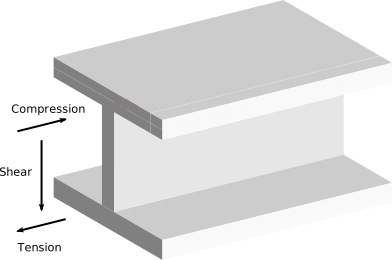
\includegraphics[width=.7\textwidth]{PIC/CH05/SFA}
\end{figure}
%\begin{figure}[H]
%\centering\footnotesize
%\includegraphics[scale=.8]{PIC/CH05/SHEAR1}\hfill
%\includegraphics[scale=.8]{PIC/CH05/SHEAR2}
%\caption{Stress equilibrium \citep{Hibbeler2016}}
%\end{figure}
\subsubsection{Horizontal Shear}
The shear stress on the longitudinal cut (light grey) needs to equilibrate the normal stress on the free body. According to stress equilibrium of a 2D plane, the shear stress on the section (dark grey) is assumed to be equal to that on the longitudinal cut (light grey).

The horizontal shear stress is mostly in flanges. Due to symmetry, it is self-equilibrating. The horizontal shear stress on web is often negligible for thin--walled sections.
\begin{figure}[H]
\centering
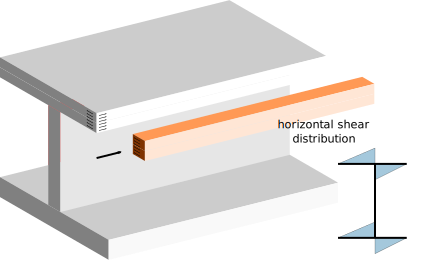
\includegraphics[width=.8\textwidth]{PIC/CH05/SFB}
\caption{Horizontal shear of free body cut on flange}
\end{figure}
\subsubsection{Vertical Shear}
For vertical shear stress, similar analysis can be performed.
\begin{figure}[H]
\centering
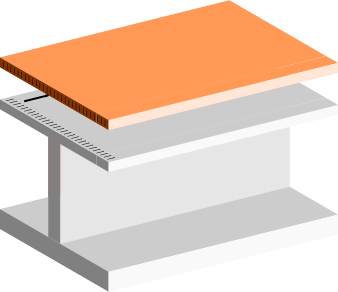
\includegraphics[width=.7\textwidth]{PIC/CH05/SFC}
\caption{Vertical shear of free body cut on flange}
\end{figure}
\begin{figure}[H]
\centering
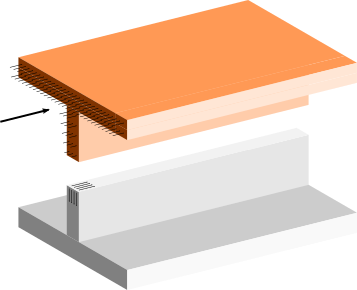
\includegraphics[width=.7\textwidth]{PIC/CH05/SFD}
\caption{Vertical shear of free body cut on web}
\end{figure}
The vertical shear in the web carries almost all of the applied shear force to a section. The flanges carry the majority of the bending (normal stress). The vertical shear stress distribution is depicted in \figref{fig:vshear}. Interested readers can check \href{https://www.youtube.com/watch?v=f08Y39UiC-o}{this}\footnote{https://www.youtube.com/watch?v=f08Y39UiC-o} video for more elaborations.
%\begin{figure}[H]
%\centering\footnotesize
%\includegraphics[width=.99\textwidth]{PIC/CH05/SHEAR3}
%\includegraphics{PIC/CH05/SHEAR}
%\caption{Shear flow distribution in an I section \citep{Hibbeler2016}}
%\end{figure}
\begin{figure}[H]
\centering\footnotesize
\includegraphics{PIC/CH05/VSHEAR}
\caption{Vertical shear distribution in an I section}\label{fig:vshear}
\end{figure}
\subsection{Shear Capacity}
In practical design, we mainly consider the \textbf{vertical} shear acting on web. It is further assumed the vertical shear is uniform/constant over the depth. The shear stress can be computed using the following expression.
\begin{gather*}
q=\dfrac{VQ}{Ib}.
\end{gather*}

A flat plate unstiffened web in an I section shall satisfy
\begin{gather}
V^*\leqslant\phi{}V_v.
\end{gather}
The nominal shear capacity $V_v$ shall be determined as
\begin{gather}
V_v=\min\left(V_w,~V_b\right).
\end{gather}

The shear capacity associated with web yielding $V_w$ (\NZSSTEEL{\S~5.11.4.1}) is,
\begin{gather}
V_w=0.6f_{yw}A_w=0.6f_{yw}dt_w
\end{gather}
where $f_{yw}$ is the yield shear stress. For an unstiffened web, $A_w=dt_w$ is the area of web.

The shear capacity associated with web buckling $V_b$ (\NZSSTEEL{\S~5.11.5.1}) is,
\begin{gather}
V_b=V_w\left(\dfrac{82}{\dfrac{d_p}{t_w}\sqrt{\dfrac{f_y}{\SI{250}{\mpa}}}}\right)^2=0.6f_yA_w\left(\dfrac{82}{\dfrac{d_p}{t_w}\sqrt{\dfrac{f_y}{\SI{250}{\mpa}}}}\right)^2
\end{gather}
where $d_p$ is the depth of the deepest web panel, this is equal to the distance between the insides of the flanges, $d_1$. Note $d_1\neq{}d$ in general.

Also, \NZSSTEEL{Cl. 5.10.1.1} imposes the maximum web slenderness ratio as
\begin{gather}
\dfrac{d_p}{t_w}\sqrt{\dfrac{f_y}{\SI{250}{\mpa}}}\leqslant180.
\end{gather}
\begin{figure}[H]
\centering\footnotesize
\begin{tikzpicture}[>=latex]
\begin{axis}[
width=7cm,
height=7cm,
xtick=\empty,
ytick=\empty,
axis x line=center,
axis y line=center,
xlabel={$d_p/t_w$},
ylabel={$\phi{}V_v$},
xlabel style={right},
ylabel style={left},
xmin=0,xmax=3.5,ymin=0,ymax=1.2]
\addplot[ultra thick,domain=1:3,samples=20]{1/x/x};
\draw[ultra thick](axis cs:0,1)--(axis cs:1,1);
\draw[ultra thick](axis cs:3,0)--(axis cs:3,1/9);
\draw[<-](axis cs:.5,1.02)--(axis cs:1.2,1.15)node[fill=white]{yielding};
\draw[<-](axis cs:1.6,4/9)--(axis cs:2.5,.8)node[fill=white]{buckling};
\draw[<-](axis cs:3,.15)--(axis cs:3,.4)node[fill=white]{max $d_p/t_w$};
\node at(axis cs:.8,.2){safe region};
\end{axis}
\end{tikzpicture}\caption{Design region of shear capacity}
\end{figure}
\subsection{Interaction Between Bending and Shear}
For the majority of practical situations, we can ignore a reduction in bending strength due to shear, or a reduction in shear strength due to bending also being carried by the section. This is because the bending is carried mainly by the flanges of an I beam bending about its strong axis, the shear is resisted mainly by the web.
However, for cases in which both $V^*$ is close to $\phi{}V_v$ and $M^*$ is close to $\phi{}M_s$, a reduction in strength should be considered. Interested readers can refer to \citet{JCWRCA1971} for elaborations.

To account for such an interaction, to design a web under shear in the presence of bending moment, it shall satisfy (\NZSSTEEL{\S~5.12.2})
\begin{gather}
V^*\leqslant\phi{}V_{vm},
\end{gather}
where
\begin{gather}
V_{vm}=\left\{
\begin{array}{ll}
V_v,&\text{for~}\dfrac{M^*}{\phi{}M_s}\leqslant0.75,\\
V_v\left(2.2-1.6\dfrac{M^*}{\phi{}M_s}\right),&\text{for~}0.75<\dfrac{M^*}{\phi{}M_s}\leqslant1.
\end{array}
\right.
\end{gather}
To illustrate, the following graph can be used.
\begin{figure}[H]
\centering\footnotesize
\begin{tikzpicture}[>=latex]
\begin{axis}[
width=7cm,
height=7cm,
xtick=\empty,
ytick=\empty,
axis x line=center,
axis y line=center,
xlabel={$\dfrac{M^*}{\phi{}M_s}$},
ylabel={$\dfrac{V^*}{\phi{}V_v}$},
xlabel style={right},
ylabel style={left},
xmin=-.2,xmax=1.2,ymin=-.2,ymax=1.2]
\draw[ultra thick](axis cs:0,1)node[left]{\num{1}}--(axis cs:.75,1)--(axis cs:1,.6)--(axis cs:1,0)node[below]{\num{1}};
\draw[dashed](axis cs:0,.6)node[left]{\num{0.6}}--(axis cs:1,.6);
\draw[dashed](axis cs:.75,0)node[below]{\num{0.75}}--(axis cs:.75,1);
\end{axis}
\end{tikzpicture}\caption{Interaction between shear and moment}
\end{figure}

\begin{exmp}
Determine the maximum factored UDL, $\omega^*$, that can be applied to the previous fully restrained 310UB32.0 beam using Grade 300 steel.
\end{exmp}
\begin{solution}
\begin{itemize}
\item \textbf{flexure}\\
Given that $M^*\leqslant\phi{}M_b$ and the maximum moment at midspan
\begin{gather*}
M^*=\dfrac{\omega^*l^2}{8},
\end{gather*}
the maximum $\omega^*$ can be computed as
\begin{gather*}
\dfrac{\omega^*l^2}{8}\leqslant\phi{}M_b,\\
\omega^*\leqslant\dfrac{8}{l^2}\phi{}M_b=\dfrac{8}{\SI{3}{\meter}\times\SI{3}{\meter}}\times\SI{134.4}{\kn\meter}=\SI{119.5}{\kn\per\meter}.
\end{gather*}
\item \textbf{shear}\\
Check the factor,
\begin{gather*}
\dfrac{82}{\dfrac{d_p}{t_w}\sqrt{\dfrac{f_y}{\SI{250}{\mpa}}}}=\dfrac{82}{\dfrac{\SI{282}{\mm}}{\SI{5.5}{\mm}}\sqrt{\dfrac{\SI{320}{\mpa}}{\SI{250}{\mpa}}}}=1.41>1.
\end{gather*}
Thus yield capacity governs, that is
\begin{gather*}
V_v=0.6f_yA_w=0.6\times\SI{320}{\mpa}\times\SI{298}{\mm}\times\SI{5.5}{\mm}=\SI{314.7}{\kn}.
\end{gather*}
Then the maximum shear at ends shall satisfy
\begin{gather*}
\dfrac{\omega^*l}{2}=V^*\leqslant\phi{}V_v,\\
\omega^*\leqslant\dfrac{2}{l}\phi{}V_v=\dfrac{2}{\SI{3}{\meter}}\times0.9\times\SI{314.7}{\kn}=\SI{188.8}{\kn\per\meter}.
\end{gather*}
\begin{flushright}
$\omega^*\leqslant\SI{188.8}{\kn\per\meter}$
\end{flushright}
\end{itemize}
Thus flexure governs, the maximum $\omega^*$ is $\SI{119.5}{\kn\per\meter}$. It is noted that shear tends to govern in very short members.
\end{solution}
\section{Design for Bearing}
Modes of failure near a concentrated load are web buckling and web yielding. To compute either we need to know how the force is transferred into the web of the beam.

The design froce $R^*$ on a web shall then satisfy (\NZSSTEEL{\S~5.13.2})
\begin{gather}
R^*\leqslant\phi{}R_b=\min\left(\phi{}R_{by},~\phi{}R_{bb}\right),
\end{gather}
where $R_b$ shall be the smaller of $R_{by}$ and $R_{bb}$ as defined below.
\subsection{Force Dispersion}
Point load is an idealised concept that does not exist in practice. All loads are applied to regions of finite areas. \NZSSTEEL{\S~5.13.1} requires the dispersion of load through the flange shall be taken at a slope of 1:2.5 to the surface of the flange while the dispersion of load to the flange shall be taken at a slope of 1:1 through solid material.
\begin{figure}[H]
\centering
\includegraphics[width=.99\textwidth]{PIC/CH05/LD}
\caption{Web bearing and the load dispersion method \citep{Gorenc2015}}
\end{figure}
\begin{figure}[H]
\centering\footnotesize
\begin{tikzpicture}[ext/.pic={
\path[fill=white](-0.2,0)to[bend left](0,0.1)to[bend right](0.2,0.2)to(0.2,0)to[bend left](0,-0.1)to[bend right](-0.2,-0.2)--cycle;
\draw(-0.2,0)to[bend left](0,0.1)to[bend right](0.2,0.2) (0.2,0)to[bend left](0,-0.1)to[bend right](-0.2,-0.2);
}]
\setstructmech{fill=black!10}
\UDL{-1,.3}{1,.3}[]{.5}
\draw(-4,0)rectangle(4,.3);
\draw(-4,0)rectangle(4,-4);
\draw(-4,-4)rectangle(4,-4.3);
\draw[pattern=north west lines](5,0)rectangle(8,.3);
\draw[pattern=north west lines](5,-4)rectangle(8,-4.3);
\draw[pattern=north west lines](6.35,0)rectangle(6.65,-4);
\draw[dashed](-5,-2)--(8,-2)node[above=2mm]{N.A.};
\draw(-1,.3)--++(-2.5*.3,-.3)coordinate(A)--++(-2,-2)coordinate(C);
\draw(1,.3)--++(2.5*.3,-.3)coordinate(B)--++(2,-2)coordinate(D);
\draw[cc0066,line width=.8mm](A)--(B);
\draw[0066cc,line width=.8mm](C)--(D);
\draw[cc0066,line width=.8mm](6.35,0)--(6.65,0);
\draw[0066cc,line width=.8mm](6.35,-2)--(6.65,-2);
\draw[|<->|](-1,1.2)--(1,1.2)node[midway,fill=white]{$b_{s}$};
\draw[|<->|]($(A)-(0,.5)$)--($(B)-(0,.5)$)node[midway,fill=white]{$b_{bf}=b_s+5t_f$};
\draw[|<->|]($(C)-(0,.5)$)--($(A)-(0,2.5)$)node[midway,fill=white]{$b_{bw}=d_1/2$};
\draw[|<->|]($(A)-(0,2.5)$)--($(B)-(0,2.5)$)node[midway,fill=white]{$b_{bf}$};
\draw[|<->|]($(B)-(0,2.5)$)--($(D)-(0,.5)$)node[midway,fill=white]{$b_{bw}$};
\draw[|<->|]($(C)-(0,1)$)--($(D)-(0,1)$)node[midway,fill=white]{$b_{b}=b_{bf}+2b_{bw}=b_{bf}+d_1$};
\draw[|<->|](-4.5,-2)--++(0,2)node[midway,fill=white]{$\dfrac{d_1}{2}$};
\draw(4,-2)pic{ext};
\draw(-4,-2)pic{ext};
\draw[<-](B)--++(2,.8)coordinate(E);
\draw[<-](6.5,.1)--(E)node[fill=white]{web yielding area};
\draw[<-](D)--++(1,-1.4)coordinate(F);
\draw[<-](6.5,-2)--(F)node[fill=white]{web buckling area};
\end{tikzpicture}
\caption{Interior force}
\end{figure}
\begin{figure}[H]
\centering\input{PIC/CH05/FD2}
\caption{End force}
\end{figure}

If loading is applied from another section, then the way the force should be computed on the beam being designed in shown below.
\begin{figure}[H]
\centering\includegraphics{PIC/CH05/BEARO}\caption{Ineffective regions are ignored}
\end{figure}
\subsection{Yielding}
Web yielding will occur over the area $b_{bf}t_w$ when there is either high load or small area. The nominal bearing yield capacity of a web shall be calculated as (\NZSSTEEL{\S~5.13.3.1})
\begin{gather}
R_{by}=1.25b_{bf}t_wf_y.
\end{gather}
The factor \num{1.25} considers the following aspects:
\begin{itemize}
\item potential higher strength under compression,
\item Poisson's ratio,
\item force distribution may be conservative, and
\item triaxial stresses from flange.
\end{itemize}
\subsection{Buckling}
Web buckling is assumed to occur following the pattern as shown in absence of web stiffeners.
\begin{figure}[H]
\centering
\begin{tikzpicture}[scale=1]
\def\a{1.5}\def\b{2}
\draw[dashed](0,-\b)--++(0,2*\b);
\draw[dashed](-\a,-\b)--++(2*\a,0);
\draw[dashed](-\a,\b)--++(2*\a,0);
\setstructmech{convention=direction}
\NodalForce{0,4}[N][-N^*][N]
\draw[line width=2mm](-\a,-\b)--++(2*\a,0);
\draw[line width=2mm](-\a,\b)--++(2*\a,0);
\draw[line width=2mm](0,\b)to[out=-90,in=90](.2*\a,0)to[out=-90,in=90](0,-\b);
\draw[|<->|](-\a,-.5*\b)--++(0,\b)node[midway,fill=white]{$L_e\approx0.72d_1$};
\end{tikzpicture}
\caption{Web buckling due to bearing}
\end{figure}
The critical stress is at centre (mid height) of beam web over the area $b_bt_w$. The nominal bearing buckling capacity $R_{bb}$ is determined as the axial compression capacity using $\alpha_b=0.5$ and $k_f=1$ with slenderness ratio $L_e/r=2.5d_1/t_w$ (\NZSSTEEL{\S~5.13.4}).
\begin{gather}
R_{bb}=\alpha_cN_s=\alpha_cb_bt_wf_y.
\end{gather}
It shall be noted $f_y=f_{y,web}$ shall be taken as the yield strength of web. The slenderness ratio $L_e/r=2.5d_1/t_w$ is equivalent to considering $L_e\approx0.72d_1$. For web with size $t_w\times{}d_1$, the radius of gyration is
\begin{gather}
r=r_y=\sqrt{\dfrac{I_y}{A}}=\sqrt{\dfrac{t_w^3d_1}{12t_wd_1}}=\dfrac{t_w}{\sqrt{12}},
\end{gather}
this leads to
\begin{gather}
\dfrac{L_e}{r}=\dfrac{0.72d_1}{t_w/\sqrt{12}}\approx2.5\dfrac{d_1}{t_w}.
\end{gather}
The above is valid for I sections. Different equations are needed for other sections. Interested readers can refer to \NZSSTEEL{\S~5.14}.
\subsection{Web Stiffener}
If the requirements for yielding or buckling above are not satisfied then load bearing stiffeners must be provided. They can be provided in one or both sides, should fit tightly, and may or may not extend over the whole depth.
\begin{figure}[H]
\centering\footnotesize
\begin{tikzpicture}
\begin{scope}[xshift=4cm]
\draw[pattern=north west lines](0,0)rectangle(3,.3);
\draw[pattern=north west lines](0,-4)rectangle(3,-4.3);
\draw[pattern=north west lines](1.35,0)rectangle(1.65,-4);
\draw[draw=cc0066,line width=.8mm,fill=cc0066!20](.4,0)rectangle(1.35,-4);
\draw[draw=cc0066,line width=.8mm,fill=cc0066!20](2.6,0)rectangle(1.65,-4);
\node at(1.5,-5.5)[align=center]{both sided\\full height\\stiffener};
\end{scope}
\begin{scope}[xshift=9cm]
\draw[pattern=north west lines](0,0)rectangle(3,.3)node[below=4mm]{in compression};
\draw[pattern=north west lines](0,-4)rectangle(3,-4.3)node[above=4mm]{in tension};
\draw[pattern=north west lines](1.35,0)rectangle(1.65,-4);
\draw[draw=cc0066,line width=.8mm,fill=cc0066!20](.4,0)rectangle(1.35,-3);
\node at(1.5,-5.5)[align=center]{single sided\\partial height stiffener\\to avoid fatigure fracture};
\end{scope}
\node at(0,-3){\includegraphics[height=6cm]{PIC/CH05/STIFFENER}};
\end{tikzpicture}
\caption{Web stiffeners}
\end{figure}
\subsubsection{Web Yielding}
The design force $R^*$ shall satisfy (\NZSSTEEL{5.14.1})
\begin{gather}
R^*\leqslant\phi{}R_{sy},
\end{gather}
where
\begin{conditions}
R_{sy}&nominal yield capacity of the stiffened web
\end{conditions}
The nominal yield capacity of the stiffened web shall be computed as
\begin{gather}
R_{sy}=R_{by}+A_sf_{ys},
\end{gather}
where
\begin{conditions}
R_{by}&nominal bearing yield capacity\\
A_s&area of the stiffener in contact with the flange\\
f_{ys}&yield stress of the stiffener
\end{conditions}
\subsubsection{Web Buckling}
The design force $R^*$ shall satisfy (\NZSSTEEL{5.14.2})
\begin{gather}
R^*\leqslant\phi{}R_{sb},
\end{gather}
where $R_{sb}$ is the nominal buckling capacity of the stiffened web which shall be determined in a way similar to compression members as follows.
\begin{gather}
R_{sb}=\alpha_cN_s=\alpha_ck_fA_nf_y.
\end{gather}
In which, $\alpha_c$ shall be computed according to \S~\ref{sec:n_c} with modified slenderness ratio $\lambda_n$ be
\begin{gather}
\lambda_n=\dfrac{L_e}{r}\sqrt{k_f}\sqrt{\dfrac{f_y}{\SI{250}{\mpa}}},
\end{gather}
using $k_f=1$, $\alpha_b=0.5$, $r$ be the radius of gyration about the neutral axis of $A_n$ parallel to web, $L_e$ be
\begin{itemize}
\item $0.7d_1$ where flanges are restrained against rotation in plane of stiffener, or
\item $d_1$ where flanges are \textbf{not} restrained against rotation in plane of stiffener.
\end{itemize}
The net area $A_n$ can be taken as the summation of the gross area of the stiffener(s) plus the effective area of the web as shown.
\begin{figure}[H]
\centering\footnotesize
\begin{tikzpicture}
\draw[dashed](-5,0)--(5,0)node[right=5mm]{bucking axis};
\node at(-4,.5){web};
\node at(1,1){stiffener};
\node at(4,1){$A_n=\text{all shaded area}$};
\draw[pattern=north west lines](-4,-.1)rectangle(4,.1);
\draw[pattern=north west lines](-.1,.1)rectangle(.1,1);
\draw[pattern=north west lines](-.1,-.1)rectangle(.1,-1);
\draw[|<->|](-4,-1.2)--++(4,0)node[midway,fill=white]{$b_e$};
\draw[|<->|](0,-1.2)--++(4,0)node[midway,fill=white]{$b_e$};
\draw[|<->|](-.5,.1)--(-.5,1)node[midway,fill=white]{$b_{es}$};
\draw[|<->|](-.1,1.2)--(.1,1.2)node[midway,above=2mm]{$t_s$};
\draw[|<->|](-4.4,-.1)--++(0,.2)node[midway,left=2mm,fill=white]{$t_w$};
\end{tikzpicture}
\caption{Plan view at web buckling surface}
\end{figure}

The effective width $b_e$ of each side of the stiffener(s) centreline shall be the smaller of $17.5t_w\sqrt{\frac{\SI{250}{\mpa}}{f_y}}$ and $s/2$ where $s$ is the stiffener spacing.

The width to thickness ratio of any stiffener element should also satisfy
\begin{gather}
\dfrac{b_{es}}{t_s}\sqrt{\dfrac{f_{ys}}{\SI{250}{\mpa}}}\leqslant15,
\end{gather}
where $b_{es}$ is the width of stiffener, $t_s$ is the thickness of stiffener and $f_{ys}$ is the yield strength of stiffener.

It is easiest to prevent buckling problems by providing a sufficiently large support.
\begin{exmp}\href{run:./WORKSHEET/CH05/EX5.BUDL.sm}{Worksheet} Bearing Design

If a $\SI{3}{\meter}$ long Grade 300 310UB32.0 beam subject to UDL of $\omega=\SI{119}{\kn\per\meter}$ is supported on a $\SI{100}{\mm}$ wide plate at either end, and if the beam continues $\SI{120}{\mm}$ beyond the centre of the support, is it satisfactory?
\end{exmp}
\begin{solution}
\begin{figure}[H]
\footnotesize
\begin{tikzpicture}[scale=2,ext/.pic={
\path[fill=exmpbg](-0.2,0)to[bend left](0,0.1)to[bend right](0.2,0.2)to(0.2,0)to[bend left](0,-0.1)to[bend right](-0.2,-0.2)--cycle;
\draw(-0.2,0)to[bend left](0,0.1)to[bend right](0.2,0.2) (0.2,0)to[bend left](0,-0.1)to[bend right](-0.2,-0.2);
}]
\draw[dashed](.6,-.2)--++(0,1.3);
\draw(0,0)rectangle(4,.1);
\draw(0,.1)rectangle(4,.9);
\draw(0,.9)rectangle(4,1);
\draw[fill=black](.35,-.1)rectangle(.85,0);
\draw[|<->|](0,.6)--(.6,.6)node[midway,above=1mm,fill=exmpbg]{\SI{120}{\mm}};
\draw[|<->|](.35,.3)--(.85,.3)node[midway,above=1mm,fill=exmpbg]{\SI{100}{\mm}};
\draw(4,.5)pic{ext};
\draw[<-,ultra thick](.6,-.3)--++(0,-.4)node[below]{$V^*$};
\end{tikzpicture}
\end{figure}
For force dispersion,
\begin{gather*}
b_{bf}=b_s+5t_f=\SI{100}{\mm}+5\times\SI{8}{\mm}=\SI{140}{\mm},\\
b_{bw}=\dfrac{d_1}{2}=\SI{141}{\mm},\\
b_0=\SI{120}{\mm}-0.5\times\SI{140}{\mm}=\SI{50}{\mm},\\
\begin{split}
b_b&=\min\left(b_{bf}+2b_{bw},b_{bf}+b_{bw}+b_0\right)\\
&=\min\left(\SI{140}{\mm}+2\times\SI{141}{\mm},\SI{140}{\mm}+\SI{141}{\mm}+\SI{50}{\mm}\right)\\
&=\SI{331}{\mm}.
\end{split}
\end{gather*}
The shear demand is
\begin{gather*}
V^*=\dfrac{\omega{}L}{2}=\dfrac{\SI{119}{\kn\per\meter}\times\SI{3}{\meter}}{2}=\SI{178.5}{\kn}.
\end{gather*}
For web yielding,
\begin{align*}
\phi{}R_{by}&=\phi{}1.25b_{bf}t_wf_y\\
&=0.9\times1.25\times\SI{140}{\mm}\times\SI{5.5}{\mm}\times\SI{320}{\mpa}\\
&=\SI{277.2}{\kn}>V^*=\SI{178.5}{\kn}.
\end{align*}
For web buckling,
\begin{gather*}
\dfrac{L_e}{r}=2.5\dfrac{d_1}{t_w}=2.5\times\dfrac{282}{5.5}=128.2,\\
\lambda_n=\dfrac{L_e}{r}\sqrt{k_f}\sqrt{\dfrac{f_y}{\SI{250}{\mpa}}}=128.2\times1\times\sqrt{\dfrac{\SI{320}{\mpa}}{\SI{250}{\mpa}}}=145.
\end{gather*}
Using $\alpha_b=0.5$, one can obtain $\alpha_c=0.288$. Thus,
\begin{align*}
\phi{}R_{bb}&=\phi{}\alpha_cb_bt_wf_y\\
&=0.9\times0.288\times\SI{331}{\mm}\times\SI{5.5}{\mm}\times\SI{320}{\mpa}\\
&=\SI{151.0}{\kn}<V^*=\SI{178.5}{\kn}.
\end{align*}
\begin{flushright}
NOT GOOD
\end{flushright}
It can be seen than web buckling governs and $V^*>\phi{}R_{bb}$. One can increase $b_s$, extend beam, or add stiffener to avoid buckling failure.
\end{solution}
\section{Biaxial Loading}
The biaxial bending can be decomposed into strong axis and weak axis components.
\begin{figure}[H]
\centering\begin{tikzpicture}
\newcommand{\Base}{
\draw[dashed](-1,0)--(1,0)node[fill=white]{$x$};
\draw[dashed](0,-1.5)node[fill=white]{$y$}--++(0,3);
\draw[line width=2mm](0,-1)--++(0,2);
\draw[line width=2mm](-1,-1)--++(2,0)(-1,1)--++(2,0);}
\begin{scope}[rotate=30]
\Base
\end{scope}
\begin{scope}[xshift=5cm]
\Base
\end{scope}
\begin{scope}[xshift=10cm]
\Base
\end{scope}
\node at(2.5,0){\LARGE$=$};
\node at(7.5,0){\LARGE$+$};
\draw[line width=.8mm,->>](0,3)node[above]{$M^*=\sqrt{\left(M_x^*\right)^2+\left(M_y^*\right)^2}$}--(0,2);
\draw[line width=.8mm,->>](5,3)node[above]{$M_y^*$}--(5,2);
\draw[line width=.8mm,->>](12.5,0)node[right]{$M_x^*$}--++(-1,0);
\end{tikzpicture}\caption{Decomposition of biaxial moment into $x$ and $y$ components}
\end{figure}
In absence of axial force, \NZSSTEEL{Cl.~8.4.5.1} requires
\begin{align}
\left(\dfrac{M^*_x}{\phi{}M_{cx}}\right)^{1.4}+\left(\dfrac{M^*_y}{\phi{}M_{cy}}\right)^{1.4}\leqslant1.0,
\end{align}
where major axis bending occurs about the $x$-axis and minor axis bending ocurs about the $y$-axis. Furthermore, $M_{cx}=\min\left(M_{sx}~,M_{bx}\right)$ for the major (strong) axis and $M_{cy}=M_{sy}$ for the minor (weak) axis. FLT buckling does \textbf{not} occur for bending about weak axis.
\begin{figure}[H]
\centering\footnotesize
\begin{tikzpicture}
\begin{axis}[
width=7cm,height=7cm,
axis x line=middle,
axis y line=middle,
axis equal,
xlabel=$\dfrac{M^*_x}{\phi{}M_{cx}}$,
ylabel=$\dfrac{M^*_y}{\phi{}M_{cy}}$,
x label style={at={(axis description cs:0.5,-0.05)},anchor=north},
y label style={at={(axis description cs:-0.15,.5)},anchor=south},
xmin=-.1,
ymin=-.1,
xmax=1.1,
ymax=1.1,
]
\addplot[domain=0:.61,samples=100,line width=.8mm]({x},{(1-x^1.4)^(5/7)});
\addplot[domain=0:.61,samples=100,line width=.8mm]({(1-x^1.4)^(5/7)},{x});
\addplot[domain=0:1,samples=2,dashed]({x},{1-x});
\end{axis}
\end{tikzpicture}\caption{Envelop of biaxial moments}
\end{figure}
\clearpage
\begin{exmp}
Biaxial Design

The factored moments on a beam, including self--weight, are $M^*_x=\SI{200}{\kn\meter}$ and $M^*_y=\SI{50}{\kn\meter}$. Select a Grade 300 UB section to resist these moments assuming full lateral support of the compression flange.
\end{exmp}
\begin{solution}
Try 460UB74.6,
\begin{align*}
&\left(\dfrac{M^*_x}{\phi{}M_{cx}}\right)^{1.4}+\left(\dfrac{M^*_y}{\phi{}M_{cy}}\right)^{1.4}\\
=&\left(\dfrac{M^*_x}{\phi{}M_{sx}}\right)^{1.4}+\left(\dfrac{M^*_y}{\phi{}M_{sy}}\right)^{1.4}\\
=&\left(\dfrac{\SI{200}{\kn\meter}}{\SI{448.2}{\kn\meter}}\right)^{1.4}+\left(\dfrac{\SI{50}{\kn\meter}}{\SI{70.7}{\kn\meter}}\right)^{1.4}\\
=&0.939<1.0
\end{align*}
Since the member is fully supported, $M_{cx}=M_{sx}$ and $M_{cy}=M_{sy}$.

For unbraced members, $M_{cx}=M_{bx}$ which depends on $\alpha_m$, unbraced length, etc.
\end{solution}
\begin{sidewaystable}[p]
\centering\scriptsize\setlength{\tabcolsep}{2pt}\renewcommand{\arraystretch}{1.4}
\caption{Design load capacity table for members subject to strong axis bending ($\alpha_m=1.0$)}\label{tab:ub_strong_bending}
\begin{tabular}{r|c|c|ccccccccccccccccccccccccccc}
	\toprule
	                                                                                                      \multicolumn{30}{c}{\Large{}Grade 300 UB \textbf{Strong} Axis Bending ($\alpha_m=1.0$)}                                                                                                       \\ \midrule
	                    & $\phi{}M_{sx}$ (\si{\kn}) & $\phi{}M_{sy}$ (\si{\kn}) &                                                                                  \multicolumn{27}{c}{$\alpha_s\phi{}M_s$ (\si{\kn})}                                                                                  \\
	$L_e$ (\si{\meter}) &           0.00            &           0.00            & 1.00  & 1.25  & 1.50  & 1.75  & 2.00  & 2.25  & 2.50  & 2.75  & 3.00  & 3.25  & 3.50  & 3.75  & 4.00  & 4.25  & 4.50  & 4.75  & 5.00  & 5.50  & 6.00  & 6.50  & 7.00  & 7.50  & 8.00  & 8.50  & 9.00  & 9.50  & 10.00 \\ \midrule
	           610UB125 &           927.4           &           129.8           & 927.4 & 926.1 & 910.3 & 892.3 & 872.2 & 850.5 & 827.3 & 803.0 & 777.9 & 752.3 & 726.4 & 700.4 & 674.7 & 649.3 & 624.5 & 600.3 & 577.0 & 532.8 & 492.4 & 455.7 & 422.7 & 393.2 & 366.7 & 343.1 & 321.9 & 302.9 & 285.8 \\
	           610UB113 &           829.1           &           113.7           & 829.1 & 826.9 & 812.3 & 795.6 & 777.1 & 756.9 & 735.4 & 712.8 & 689.5 & 665.6 & 641.5 & 617.3 & 593.4 & 569.8 & 546.7 & 524.2 & 502.5 & 461.7 & 424.5 & 390.9 & 360.9 & 334.1 & 310.3 & 289.1 & 270.2 & 253.4 & 238.4 \\
	           610UB101 &           783.0           &           104.2           & 783.0 & 777.4 & 762.1 & 744.7 & 725.3 & 704.2 & 681.8 & 658.3 & 634.1 & 609.4 & 584.5 & 559.7 & 535.3 & 511.3 & 488.0 & 465.4 & 443.8 & 403.5 & 367.3 & 335.2 & 306.8 & 281.8 & 259.9 & 240.6 & 223.6 & 208.6 & 195.3 \\
	          530UB92.4 &           639.9           &           92.3            & 639.9 & 631.3 & 617.3 & 601.5 & 584.0 & 565.3 & 545.5 & 525.1 & 504.2 & 483.2 & 462.3 & 441.7 & 421.7 & 402.2 & 383.5 & 365.7 & 348.7 & 317.4 & 289.6 & 265.2 & 243.8 & 225.0 & 208.5 & 194.0 & 181.3 & 169.9 & 159.9 \\
	          530UB82.0 &           558.9           &           78.0            & 558.9 & 550.2 & 537.5 & 523.0 & 507.1 & 489.9 & 471.8 & 453.1 & 434.0 & 414.8 & 395.6 & 376.8 & 358.5 & 340.8 & 323.8 & 307.6 & 292.3 & 264.1 & 239.4 & 217.8 & 199.0 & 182.6 & 168.4 & 156.0 & 145.1 & 135.5 & 127.0 \\
	          460UB82.1 &           496.8           &           78.8            & 496.8 & 486.4 & 474.3 & 460.6 & 445.8 & 430.0 & 413.7 & 397.0 & 380.2 & 363.5 & 347.2 & 331.3 & 315.9 & 301.3 & 287.3 & 274.1 & 261.6 & 238.9 & 218.9 & 201.4 & 186.1 & 172.7 & 160.9 & 150.5 & 141.3 & 133.1 & 125.8 \\
	          460UB74.6 &           448.2           &           70.7            & 447.9 & 438.4 & 427.2 & 414.6 & 400.9 & 386.3 & 371.1 & 355.5 & 339.9 & 324.3 & 309.1 & 294.2 & 279.9 & 266.3 & 253.3 & 241.0 & 229.5 & 208.4 & 190.1 & 174.1 & 160.2 & 148.1 & 137.5 & 128.2 & 120.0 & 112.8 & 106.3 \\
	          460UB67.1 &           399.6           &           62.1            & 399.0 & 390.2 & 379.9 & 368.3 & 355.7 & 342.2 & 328.1 & 313.7 & 299.2 & 284.8 & 270.6 & 256.9 & 243.6 & 231.0 & 219.0 & 207.7 & 197.1 & 177.9 & 161.2 & 146.8 & 134.4 & 123.6 & 114.3 & 106.1 & 99.0  & 92.7  & 87.1  \\
	          410UB59.7 &           324.0           &           54.8            & 322.3 & 314.7 & 305.8 & 295.8 & 285.0 & 273.5 & 261.7 & 249.8 & 237.8 & 226.1 & 214.6 & 203.6 & 193.1 & 183.2 & 173.8 & 164.9 & 156.7 & 141.9 & 129.0 & 118.0 & 108.4 & 100.2 & 93.0  & 86.7  & 81.1  & 76.2  & 71.9  \\
	          410UB53.7 &           305.3           &           49.8            & 302.2 & 294.2 & 284.9 & 274.4 & 263.1 & 251.2 & 239.0 & 226.7 & 214.4 & 202.4 & 190.9 & 179.8 & 169.4 & 159.6 & 150.4 & 141.9 & 134.0 & 120.0 & 108.1 & 97.9  & 89.3  & 82.0  & 75.7  & 70.2  & 65.4  & 61.2  & 57.5  \\
	          360UB56.7 &           272.7           &           52.1            & 270.8 & 264.1 & 256.4 & 247.9 & 238.7 & 229.2 & 219.3 & 209.5 & 199.7 & 190.2 & 180.9 & 172.1 & 163.7 & 155.7 & 148.2 & 141.2 & 134.7 & 122.8 & 112.6 & 103.6 & 95.9  & 89.1  & 83.2  & 77.9  & 73.3  & 69.2  & 65.5  \\
	          360UB50.7 &           242.2           &           45.4            & 240.2 & 234.1 & 227.0 & 219.2 & 210.7 & 201.8 & 192.7 & 183.5 & 174.4 & 165.6 & 157.0 & 148.8 & 141.0 & 133.6 & 126.7 & 120.3 & 114.3 & 103.6 & 94.3  & 86.3  & 79.5  & 73.5  & 68.4  & 63.8  & 59.8  & 56.3  & 53.1  \\
	          360UB44.7 &           221.8           &           40.3            & 218.9 & 212.8 & 205.8 & 197.9 & 189.4 & 180.5 & 171.4 & 162.3 & 153.3 & 144.5 & 136.1 & 128.2 & 120.6 & 113.6 & 107.1 & 101.0 & 95.4  & 85.5  & 77.1  & 70.0  & 64.0  & 58.8  & 54.3  & 50.5  & 47.1  & 44.1  & 41.5  \\
	          310UB46.2 &           196.8           &           44.0            & 195.2 & 190.3 & 184.6 & 178.4 & 171.7 & 164.8 & 157.7 & 150.6 & 143.6 & 136.8 & 130.2 & 124.0 & 118.0 & 112.4 & 107.2 & 102.2 & 97.6  & 89.2  & 82.0  & 75.7  & 70.2  & 65.4  & 61.1  & 57.4  & 54.1  & 51.1  & 48.4  \\
	          310UB40.4 &           182.3           &           40.0            & 179.9 & 174.9 & 169.1 & 162.7 & 155.9 & 148.8 & 141.5 & 134.3 & 127.2 & 120.3 & 113.8 & 107.5 & 101.7 & 96.2  & 91.0  & 86.3  & 81.9  & 74.1  & 67.4  & 61.6  & 56.7  & 52.5  & 48.8  & 45.6  & 42.7  & 40.2  & 38.0  \\
	          310UB32.0 &           134.5           &           25.0            & 130.7 & 126.0 & 120.7 & 114.8 & 108.7 & 102.4 & 96.1  & 90.0  & 84.1  & 78.5  & 73.3  & 68.5  & 64.1  & 60.0  & 56.3  & 52.9  & 49.9  & 44.5  & 40.1  & 36.4  & 33.3  & 30.6  & 28.4  & 26.4  & 24.7  & 23.2  & 21.8  \\
	          250UB37.3 &           140.0           &           33.4            & 136.6 & 132.1 & 127.0 & 121.5 & 115.9 & 110.1 & 104.4 & 98.9  & 93.6  & 88.6  & 83.9  & 79.5  & 75.4  & 71.6  & 68.1  & 64.8  & 61.8  & 56.4  & 51.9  & 47.9  & 44.5  & 41.5  & 38.8  & 36.5  & 34.5  & 32.6  & 30.9  \\
	          250UB31.4 &           113.8           &           26.3            & 110.6 & 106.8 & 102.4 & 97.6  & 92.6  & 87.5  & 82.5  & 77.6  & 73.0  & 68.6  & 64.4  & 60.6  & 57.0  & 53.8  & 50.8  & 48.0  & 45.5  & 41.1  & 37.4  & 34.3  & 31.6  & 29.3  & 27.3  & 25.5  & 24.0  & 22.6  & 21.4  \\
	          250UB25.7 &           91.9            &           17.8            & 86.9  & 82.7  & 78.0  & 73.1  & 68.2  & 63.4  & 58.8  & 54.5  & 50.5  & 46.9  & 43.7  & 40.7  & 38.1  & 35.7  & 33.5  & 31.6  & 29.9  & 26.9  & 24.4  & 22.3  & 20.5  & 19.0  & 17.7  & 16.6  & 15.6  & 14.7  & 13.9  \\
	          200UB29.8 &           91.0            &           24.9            & 87.9  & 84.6  & 81.0  & 77.2  & 73.3  & 69.5  & 65.8  & 62.2  & 58.9  & 55.8  & 52.8  & 50.1  & 47.6  & 45.3  & 43.2  & 41.2  & 39.4  & 36.2  & 33.4  & 31.0  & 28.8  & 27.0  & 25.4  & 23.9  & 22.6  & 21.4  & 20.4  \\
	          200UB25.4 &           74.6            &           19.8            & 71.7  & 68.8  & 65.7  & 62.3  & 58.8  & 55.4  & 52.1  & 48.9  & 46.0  & 43.2  & 40.7  & 38.3  & 36.2  & 34.2  & 32.4  & 30.7  & 29.2  & 26.6  & 24.3  & 22.4  & 20.8  & 19.3  & 18.1  & 17.0  & 16.0  & 15.2  & 14.4  \\
	          200UB22.3 &           65.4            &           17.4            & 62.9  & 60.4  & 57.6  & 54.6  & 51.5  & 48.4  & 45.4  & 42.5  & 39.8  & 37.3  & 35.0  & 32.8  & 30.9  & 29.1  & 27.5  & 26.0  & 24.6  & 22.3  & 20.3  & 18.6  & 17.2  & 16.0  & 14.9  & 14.0  & 13.1  & 12.4  & 11.7  \\
	          200UB18.2 &           51.8            &            9.9            & 46.7  & 43.4  & 40.0  & 36.7  & 33.6  & 30.8  & 28.2  & 25.9  & 23.9  & 22.1  & 20.5  & 19.1  & 17.9  & 16.8  & 15.8  & 14.9  & 14.1  & 12.8  & 11.7  & 10.7  &  9.9  &  9.2  &  8.6  &  8.1  &  7.6  &  7.2  &  6.9  \\
	          180UB22.2 &           56.2            &           11.7            & 50.2  & 47.0  & 43.7  & 40.7  & 37.9  & 35.3  & 33.0  & 30.9  & 29.0  & 27.3  & 25.8  & 24.4  & 23.1  & 22.0  & 20.9  & 20.0  & 19.1  & 17.5  & 16.2  & 15.0  & 14.0  & 13.2  & 12.4  & 11.7  & 11.1  & 10.5  & 10.0  \\
	          180UB18.1 &           45.2            &            9.4            & 40.1  & 37.2  & 34.3  & 31.5  & 29.0  & 26.7  & 24.7  & 22.8  & 21.2  & 19.8  & 18.5  & 17.4  & 16.4  & 15.5  & 14.7  & 13.9  & 13.3  & 12.1  & 11.1  & 10.3  &  9.6  &  8.9  &  8.4  &  7.9  &  7.5  &  7.1  &  6.7  \\
	          180UB16.1 &           39.7            &            8.2            & 35.0  & 32.4  & 29.7  & 27.1  & 24.8  & 22.7  & 20.8  & 19.1  & 17.7  & 16.4  & 15.3  & 14.3  & 13.4  & 12.6  & 11.9  & 11.3  & 10.7  &  9.7  &  8.9  &  8.2  &  7.6  &  7.1  &  6.7  &  6.3  &  5.9  &  5.6  &  5.3  \\
	          150UB18.0 &           38.9            &            7.7            & 33.2  & 30.6  & 28.3  & 26.2  & 24.2  & 22.5  & 21.0  & 19.7  & 18.5  & 17.4  & 16.4  & 15.5  & 14.7  & 14.0  & 13.3  & 12.7  & 12.1  & 11.2  & 10.3  &  9.6  &  8.9  &  8.4  &  7.9  &  7.4  &  7.1  &  6.7  &  6.4  \\
	          150UB14.0 &           29.4            &            5.7            & 24.4  & 22.2  & 20.1  & 18.3  & 16.6  & 15.2  & 14.0  & 12.9  & 12.0  & 11.1  & 10.4  &  9.8  &  9.2  &  8.7  &  8.2  &  7.8  &  7.5  &  6.8  &  6.2  &  5.8  &  5.4  &  5.0  &  4.7  &  4.4  &  4.2  &  4.0  &  3.8  \\ \bottomrule
\end{tabular}
\end{sidewaystable}
\begin{sidewaystable}[p]
\centering\footnotesize\setlength{\tabcolsep}{2pt}\renewcommand{\arraystretch}{1.4}
\caption{Design load capacity table for members subject to strong axis bending ($\alpha_m=1.0$)}\label{tab:uc_strong_bending}
\begin{tabular}{r|c|c|cccccccccccccccccccccccc}
	\toprule
	                                                                                          \multicolumn{27}{c}{\Large{}Grade 300 UC \textbf{Strong} Axis Bending ($\alpha_m=1.0$)}                                                                                           \\ \midrule
	                    & $\phi{}M_{sx}$ (\si{\kn}) & $\phi{}M_{sy}$ (\si{\kn}) &                                                                      \multicolumn{24}{c}{$\alpha_s\phi{}M_s$ (\si{\kn})}                                                                      \\
	$L_e$ (\si{\meter}) &           0.00            &           0.00            & 1.00  & 1.50  & 2.00  & 2.50  & 3.00  & 3.50  & 4.00  & 4.50  & 5.00  & 6.00  & 7.00  & 8.00  & 9.00  & 10.00 & 11.00 & 12.00 & 13.00 & 14.00 & 15.00 & 16.00 & 17.00 & 18.00 & 19.00 & 20.00 \\ \midrule
	           310UC158 &           675.4           &           304.9           & 675.4 & 675.4 & 672.9 & 659.2 & 644.3 & 628.7 & 612.8 & 597.0 & 581.4 & 551.4 & 523.3 & 497.0 & 472.7 & 450.2 & 429.2 & 409.8 & 391.8 & 375.0 & 359.4 & 344.9 & 331.3 & 318.6 & 306.7 & 295.6 \\
	                137 &           579.6           &           262.1           & 579.6 & 579.6 & 576.7 & 564.2 & 550.5 & 536.0 & 521.2 & 506.3 & 491.5 & 463.0 & 436.3 & 411.6 & 388.9 & 368.0 & 348.8 & 331.3 & 315.1 & 300.2 & 286.5 & 273.8 & 262.1 & 251.2 & 241.1 & 231.7 \\
	                118 &           493.9           &           222.3           & 493.9 & 493.9 & 490.7 & 479.4 & 466.9 & 453.6 & 439.8 & 425.8 & 412.0 & 385.1 & 359.9 & 336.7 & 315.6 & 296.5 & 279.1 & 263.4 & 249.1 & 236.0 & 224.2 & 213.3 & 203.3 & 194.2 & 185.8 & 178.0 \\
	               96.8 &           421.2           &           187.4           & 421.2 & 421.2 & 416.8 & 406.2 & 394.3 & 381.4 & 368.0 & 354.3 & 340.6 & 314.1 & 289.4 & 266.9 & 246.8 & 228.8 & 212.9 & 198.8 & 186.2 & 174.9 & 164.8 & 155.8 & 147.6 & 140.2 & 133.5 & 127.3 \\
	          250UC89.5 &           310.0           &           142.9           & 310.0 & 310.0 & 302.9 & 294.0 & 284.5 & 274.7 & 264.9 & 255.4 & 246.1 & 228.7 & 213.0 & 198.8 & 186.0 & 174.5 & 164.1 & 154.7 & 146.3 & 138.6 & 131.5 & 125.1 & 119.3 & 113.9 & 108.9 & 104.3 \\
	               72.9 &           266.2           &           122.6           & 266.2 & 265.8 & 258.3 & 249.5 & 240.1 & 230.2 & 220.3 & 210.6 & 201.2 & 183.7 & 168.1 & 154.4 & 142.4 & 131.8 & 122.5 & 114.4 & 107.1 & 100.7 & 94.9  & 89.7  & 85.0  & 80.8  & 76.9  & 73.4  \\
	          200UC59.5 &           177.1           &           80.7            & 177.1 & 173.6 & 167.0 & 159.8 & 152.6 & 145.5 & 138.7 & 132.2 & 126.2 & 115.2 & 105.6 & 97.3  & 90.0  & 83.6  & 78.0  & 73.0  & 68.5  & 64.5  & 60.9  & 57.7  & 54.8  & 52.1  & 49.7  & 47.5  \\
	               52.2 &           153.9           &           70.2            & 153.9 & 150.6 & 144.5 & 137.9 & 131.0 & 124.3 & 117.9 & 111.8 & 106.1 & 95.8  & 87.0  & 79.5  & 73.0  & 67.4  & 62.5  & 58.2  & 54.4  & 51.1  & 48.1  & 45.4  & 43.0  & 40.9  & 38.9  & 37.1  \\
	               46.2 &           133.4           &           60.2            & 133.4 & 130.3 & 124.8 & 118.8 & 112.5 & 106.3 & 100.3 & 94.6  & 89.3  & 79.9  & 71.9  & 65.2  & 59.5  & 54.6  & 50.4  & 46.7  & 43.5  & 40.7  & 38.3  & 36.1  & 34.1  & 32.3  & 30.7  & 29.3  \\
	          150UC37.2 &           83.7            &           37.0            & 83.0  & 79.0  & 74.6  & 70.3  & 66.2  & 62.3  & 58.8  & 55.5  & 52.6  & 47.3  & 42.9  & 39.1  & 35.9  & 33.1  & 30.7  & 28.6  & 26.7  & 25.1  & 23.6  & 22.3  & 21.1  & 20.0  & 19.1  & 18.2  \\
	               30.0 &           72.0            &           31.7            & 71.0  & 67.0  & 62.6  & 58.1  & 53.9  & 50.0  & 46.4  & 43.2  & 40.4  & 35.5  & 31.6  & 28.4  & 25.7  & 23.5  & 21.6  & 20.0  & 18.6  & 17.3  & 16.2  & 15.3  & 14.4  & 13.7  & 13.0  & 12.4  \\
	               23.4 &           50.7            &           21.2            & 49.9  & 46.9  & 43.5  & 39.9  & 36.5  & 33.4  & 30.6  & 28.1  & 25.9  & 22.3  & 19.5  & 17.3  & 15.5  & 14.0  & 12.8  & 11.8  & 10.9  & 10.2  &  9.5  &  8.9  &  8.4  &  7.9  &  7.5  &  7.2  \\
	          100UC14.8 &           21.4            &            9.9            & 20.0  & 18.3  & 16.7  & 15.3  & 14.0  & 12.9  & 12.0  & 11.1  & 10.4  &  9.1  &  8.1  &  7.3  &  6.6  &  6.0  &  5.5  &  5.1  &  4.7  &  4.4  &  4.1  &  3.9  &  3.7  &  3.5  &  3.3  &  3.2  \\ \bottomrule
\end{tabular}
\end{sidewaystable}
\begin{figure}[p]
\centering
\includegraphics[width=.99\textwidth]{REF/UB.STRONG.MS}
\end{figure}
\begin{figure}[p]
\centering
\includegraphics[width=.99\textwidth]{REF/UC.STRONG.MS}
\end{figure}